%=======================================================================
%  Phase 2 Comprehensive Theory Paper
%  NSE AI Options Bot  --  compile with:  pdflatex -> pdflatex
%  (run pdflatex twice so the table of contents and references settle)
%=======================================================================
\documentclass[11pt,a4paper]{article}

\usepackage[margin=1in]{geometry}
\usepackage{amsmath,amssymb,amsthm}
\usepackage{booktabs}
\usepackage{graphicx}
\usepackage{float}
\usepackage{caption}
\usepackage{xcolor}
\usepackage{listings}
\usepackage{algorithm}
\usepackage{algpseudocode}
\usepackage{longtable}
\usepackage{array}
\usepackage{tikz}
\usetikzlibrary{positioning,arrows.meta,fit,backgrounds}
\usepackage[hidelinks,breaklinks=true]{hyperref}
\usepackage{url}

% ---- convenience macros ------------------------------------------------
\newcommand{\rs}{Rs.\,}                 % rupee prefix (pdflatex-safe)
\newcommand{\code}[1]{\texttt{#1}}
\newcommand{\Pup}{P(\text{UP})}
\graphicspath{{figures/}}

% ---- listings style ----------------------------------------------------
\definecolor{codegray}{gray}{0.95}
\definecolor{codekw}{rgb}{0.13,0.29,0.53}
\definecolor{codecm}{rgb}{0.25,0.50,0.35}
\definecolor{codestr}{rgb}{0.58,0.20,0.20}
\lstdefinestyle{py}{
  language=Python,
  backgroundcolor=\color{codegray},
  basicstyle=\ttfamily\footnotesize,
  keywordstyle=\color{codekw}\bfseries,
  commentstyle=\color{codecm}\itshape,
  stringstyle=\color{codestr},
  numbers=left, numberstyle=\tiny\color{gray}, numbersep=6pt,
  showstringspaces=false, breaklines=true, frame=single, framerule=0.2pt,
  captionpos=b, columns=flexible, xleftmargin=12pt,
}
\lstset{style=py}

\title{\textbf{Phase 2 Comprehensive Theory Paper:\\
Cost-Aware Walk-Forward Validation, Probability Calibration\\
and Risk Management of an AI-Driven NSE BankNifty\\
Options Trading System}}

\author{Anubhaw Raj \and Subham Singh \and Harsh Raj Sharma \and Nirban Das}
\date{\today}

\begin{document}
\maketitle

\begin{abstract}
Phase 1 of this project established a momentum-driven Gradient Boosting classifier for
NSE BankNifty options, executed through a single-position state machine, and demonstrated
it on one trading day. This paper documents Phase 2: the transition of that proof of
concept into a \emph{measurement instrument}. We report four classes of contribution.
First, \textbf{correctness}: we identify and repair a label-construction defect in the
Phase 1 pipeline in which the ``future price'' of a contract could be drawn from a
\emph{different} contract, and we add a time-gap guard and a deadband so that labels
describe tradeable moves rather than one-tick noise. Second, \textbf{friction}: we derive
a complete Indian options transaction-cost model (brokerage, Securities Transaction Tax,
exchange transaction charge, SEBI turnover fee, stamp duty, Goods and Services Tax and
per-side slippage) and show that it implies a \emph{break-even move} of roughly
$1.0\%$--$3.0\%$ of premium per round trip, a quantity that dominates strategy design.
Third, \textbf{statistical scale}: we build a Parquet feature store over approximately
1{,}200 trading days (2020--2024) and a rolling walk-forward engine that re-fits the
model daily, calibrates its probabilities by isotonic regression on a held-out fold,
selects the entry threshold by simulating post-cost profit on that fold, and abstains
entirely on days for which no edge is measurable. Fourth, \textbf{risk}: we add a
risk manager providing intrabar stops and targets, conviction-based position sizing,
daily loss limits and a volatility-regime gate, and we ablate each component on two
independent years. The headline empirical result is negative and is reported as such:
full-year 2020 net profit and loss improved from \rs$-349{,}791$ (4{,}706 trades) to
\rs$-9{,}983$ (276 trades), a $35\times$ reduction in loss, but the strategy is not
profitable after costs; gross profit before charges turns slightly positive at a
15-minute horizon while charges remain approximately \rs$57$ per trade, of which
\rs$40$ is flat brokerage. We further show that tight ($12\%$) intrabar stops destroyed
approximately \rs$116{,}000$ across 2020--2021 by harvesting one-minute microstructure
noise, and that conviction sizing on a zero-edge signal amplifies loss. We conclude that
the system has reached a \emph{trade-management noise floor} of \rs$-10{,}000$ to
\rs$-16{,}000$ per year and that further progress must come from signal quality, not
from further tuning of execution parameters. We state an explicit hypothesis for the
next phase --- that the label deadband ($0.1\%$) is an order of magnitude smaller than
the cost hurdle ($\approx 1.5\%$), so the model is currently trained to predict moves
that cannot be traded profitably --- and we specify a controlled multi-algorithm
benchmark, an event/news risk layer, and a simulated-live execution loop as the next
steps. The years 2022--2024 are held out untouched.
\end{abstract}

\tableofcontents
\newpage

%=======================================================================
\section{Introduction}
%=======================================================================

\subsection{What Phase 1 established}

The Phase 1 report \cite{phase1} developed, in order: a chronologically ordered data
pipeline over 1-minute BankNifty spot and option-chain data; a feature set built from
the Black--Scholes--Merton (BSM) framework \cite{blackscholes,merton} comprising
moneyness, time to expiry, implied volatility and the Greeks; a Gradient Boosting
Machine (GBM) binary classifier predicting whether an option's premium would be higher
five minutes later; and a two-state position machine (\textsc{out}/\textsc{in}) that
traded a single at-the-money (ATM) contract so that the backtest could not manufacture
profit by trading fifty strikes at once. Phase 1 also documented two failure modes and
their repairs: \emph{theta bias}, in which a regression target caused the model to learn
the constant negative drift of option premiums, resolved by moving to binary
classification; and \emph{absolute-price overfitting}, in which the raw premium
\code{close\_opt} carried $84.8\%$ of the Gini importance, resolved by replacing price
levels with relative momentum. The final Phase 1 configuration reported $74.6\%$
directional accuracy and an execution profile of ten trades on the test day.

\subsection{What Phase 1 could not answer}

Phase 1 was a proof of concept evaluated on \emph{one} trading day, and it deliberately
deferred four questions that determine whether a strategy is real:

\begin{enumerate}
  \item \textbf{Is the label correct?} A classifier is only as meaningful as its target.
        Phase 1 constructed the target by shifting the premium series by the horizon.
        We show in Section~\ref{sec:label} that, on a frame containing thousands of
        contracts sorted by timestamp, this operation silently compares one contract's
        present with another contract's future.
  \item \textbf{Does the edge survive friction?} Phase 1 computed profit as
        $(P_{\text{exit}}-P_{\text{entry}})\times\text{lot}$, with no brokerage, no
        statutory charges and no slippage. In Indian index options these are not a
        rounding error; Section~\ref{sec:costs} shows they are the dominant term.
  \item \textbf{Does the edge survive time?} One test day cannot distinguish skill from
        luck. Walk-forward analysis over years is the accepted minimum standard
        \cite{pardo,wfowiki}.
  \item \textbf{Is the output a probability?} Thresholds such as ``enter when
        $\Pup>0.52$'' are meaningless unless the score is calibrated, i.e.\ unless
        a score of $0.7$ corresponds to a $70\%$ empirical frequency
        \cite{zadrozny,sklearncalib}.
\end{enumerate}

\subsection{Contributions of this paper}

\begin{itemize}
  \item A per-contract labelling scheme with a time-gap guard and a configurable
        deadband, together with a unit test that proves no cross-contract leakage
        (Section~\ref{sec:label}).
  \item A complete, statutory-grounded Indian options cost model, and the derivation of
        the resulting \emph{cost hurdle} --- the percentage move required to break even
        --- tabulated across premium levels and lot sizes (Section~\ref{sec:costs}).
  \item A Parquet-backed feature store and a daily-retraining walk-forward engine with
        an explicit leakage audit (Sections~\ref{sec:arch} and~\ref{sec:decision}).
  \item Isotonic probability calibration on a held-out fold, and threshold selection by
        \emph{simulated post-cost profit} rather than by accuracy or AUC, plus an
        abstention rule that declines to trade when no edge is measurable
        (Section~\ref{sec:decision}).
  \item A configurable risk layer and a two-year ablation of every component, with an
        explanation grounded in market microstructure of why tight stops lose money on
        1-minute option bars (Section~\ref{sec:risk}).
  \item An honest empirical account, including a negative headline result, a statement
        of the noise floor, and a falsifiable hypothesis for the next phase
        (Sections~\ref{sec:results}--\ref{sec:future}).
\end{itemize}

\subsection{A note on scientific posture}

The Securities and Exchange Board of India reports that $93\%$ of individual traders in
the equity derivatives segment lost money between FY22 and FY24, with aggregate losses
exceeding \rs$1.8$ lakh crore \cite{sebi}. Any student project claiming a profitable
intraday options strategy should therefore be regarded, by default, as an artefact of
measurement error until it survives friction, time and out-of-sample testing. The
purpose of Phase 2 was not to make the equity curve rise; it was to make the equity
curve \emph{trustworthy}. Where our results are negative we report them unchanged, and
we treat the reduction of loss from \rs$-349{,}791$ to \rs$-9{,}983$ as the informative
quantity, because it isolates how much of the original loss was strategy and how much
was measurement.

%=======================================================================
\section{System Architecture}\label{sec:arch}
%=======================================================================

\subsection{Design principle: one code path, three data sources}

The central architectural decision of Phase 2 is that the data feed and the broker are
\emph{interfaces}. The same signal, risk and execution code runs when the bars come from
a historical CSV replay, from a paper broker on live data, or from a live broker. This
is what allows a strategy validated on five years of history to be promoted to live
trading without rewriting the strategy. Figure~\ref{fig:arch} shows the target
architecture; the shaded blocks are implemented in Phase 2, the dashed ones are
scheduled for the phases described in Section~\ref{sec:future}.

\begin{figure}[H]
\centering
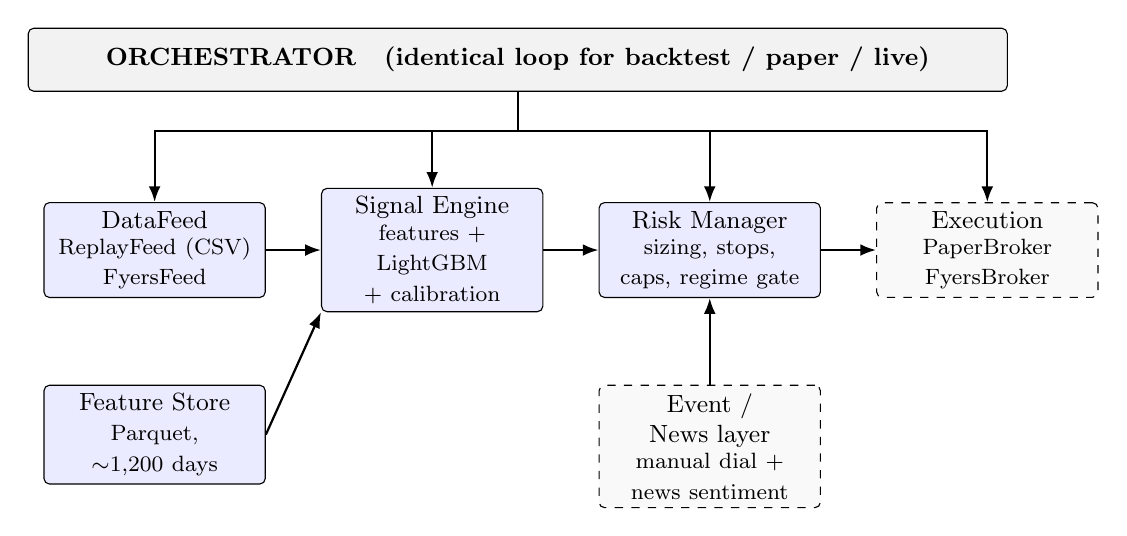
\begin{tikzpicture}[
  node distance=9mm and 7mm,
  box/.style={draw, rounded corners=2pt, align=center, minimum height=11mm,
              font=\small, inner sep=3pt, text width=26mm},
  done/.style={box, fill=blue!8},
  todo/.style={box, fill=gray!5, dashed},
  wide/.style={draw, rounded corners=2pt, align=center, font=\small\bfseries,
               minimum height=8mm, text width=122mm, fill=black!5},
  ar/.style={-{Latex[length=2mm]}, thick}
]
\node[wide] (orch) {ORCHESTRATOR \; (identical loop for backtest / paper / live)};
\node[done, below=14mm of orch.south west, anchor=north west, xshift=2mm] (feed)
  {DataFeed\\ \footnotesize ReplayFeed (CSV)\\ \footnotesize FyersFeed};
\node[done, right=of feed] (sig)
  {Signal Engine\\ \footnotesize features +\\ \footnotesize LightGBM + calibration};
\node[done, right=of sig] (risk)
  {Risk Manager\\ \footnotesize sizing, stops,\\ \footnotesize caps, regime gate};
\node[todo, right=of risk] (exec)
  {Execution\\ \footnotesize PaperBroker\\ \footnotesize FyersBroker};
\node[todo, below=11mm of risk] (evt)
  {Event / News layer\\ \footnotesize manual dial +\\ \footnotesize news sentiment};
\node[done, below=11mm of feed] (store)
  {Feature Store\\ \footnotesize Parquet, $\sim$1{,}200 days};
\draw[ar] (orch.south) -- ++(0,-5mm) -| (feed.north);
\draw[ar] (orch.south) -- ++(0,-5mm) -| (sig.north);
\draw[ar] (orch.south) -- ++(0,-5mm) -| (risk.north);
\draw[ar] (orch.south) -- ++(0,-5mm) -| (exec.north);
\draw[ar] (store.east) -- (sig.south west);
\draw[ar] (evt.north) -- (risk.south);
\draw[ar] (feed.east) -- (sig.west);
\draw[ar] (sig.east) -- (risk.west);
\draw[ar] (risk.east) -- (exec.west);
\end{tikzpicture}
\caption{Target architecture. Shaded blocks are implemented and validated in Phase 2;
dashed blocks are specified and scheduled. Because \code{DataFeed} and \code{Broker} are
interfaces, promoting the system from replay to live trading changes configuration, not
strategy code.}
\label{fig:arch}
\end{figure}

\subsection{Repository structure and configuration}

Phase 1 was a single \code{main.py} with a \code{sys.path} manipulation. Phase 2 is a
package with separated concerns (Table~\ref{tab:layout}). Every tunable quantity ---
lot sizes by effective date, cost rates, thresholds, horizons, risk limits --- lives in
\code{config/settings.yaml}, so that an experiment is described by a configuration diff
rather than by edited source code. This matters for reproducibility: each row of
\code{reports/experiments.csv} records the configuration that produced a given report
directory.

\begin{table}[H]
\centering\small
\begin{tabular}{@{}lp{9.4cm}@{}}
\toprule
\textbf{Module} & \textbf{Responsibility}\\
\midrule
\code{config/settings.yaml} & instrument specs, lot-size-by-date table, cost rates, model
and strategy parameters, risk limits\\
\code{src/config.py}        & configuration loader; \code{lot\_size\_for(cfg, instrument, date)}\\
\code{src/data/}            & raw CSV discovery and pairing (options, spot, futures)\\
\code{src/features/}        & feature engineering; Parquet feature store\\
\code{src/models/}          & LightGBM classifier, labelling, isotonic calibrator\\
\code{src/backtest/}        & cost model, position state machine, walk-forward engine, metrics\\
\code{src/risk/}            & risk manager (gates, sizing, stops)\\
\code{scripts/}             & \code{build\_features.py}, \code{run\_backtest.py}, \code{run\_walkforward.py}\\
\code{tests/}               & pytest suite: symbol parsing, labels, costs, calibration, risk\\
\code{reports/}             & one directory per run: \code{report.md}, \code{trades.csv}, \code{days.csv}, \code{equity.png}\\
\bottomrule
\end{tabular}
\caption{Package layout after the Phase 2 restructure.}
\label{tab:layout}
\end{table}

\subsection{Lot size as a function of date}

Contract size is not a constant. The NSE has repeatedly revised the BankNifty market
lot; the reduction from 25 to 15 was notified in circular NSE/FAOP/56233 dated
31 March 2023 and applied from the July 2023 monthly expiry onwards \cite{nsecircular}.
Because profit and loss scales linearly with lot size, hard-coding the Phase 1 value of
25 would misstate every trade outside its window. We therefore store a step function
\begin{equation}
L(t) \;=\; L_k \quad \text{for } t \in [d_k,\, d_{k+1}),
\end{equation}
keyed by effective date $d_k$, and resolve it per trade date. The values used are given
in Appendix~\ref{app:config}; they are approximate and are flagged in the configuration
as requiring verification against NSE circulars before any live deployment.

\subsection{The feature store}

Computing implied volatility and the Greeks is the expensive step of the pipeline: it
requires a numerical inversion of the BSM price for every row. Recomputing this on every
experiment made Phase 1-style iteration impossible at scale. Phase 2 therefore performs
the computation once per trading day and persists the result as a columnar Parquet file
\cite{parquet}:
\[
\code{data/features/\{instrument\}/\{YYYY-MM-DD\}.parquet}.
\]
Columnar storage is chosen because the walk-forward loop reads a fixed subset of
approximately thirty feature columns from each day, so column pruning avoids
deserialising the remainder. All \code{float64} columns are downcast to \code{float32}
before writing, which halves the footprint at a precision far finer than the tick size
of \rs$0.05$. Approximately 1{,}200 BankNifty trading days spanning 2020-01-01 to
2024-10-31 were built at roughly $0.8$ seconds per day with zero failures, after which a
full-year walk-forward experiment costs minutes rather than hours.

%=======================================================================
\section{Correctness: The Label-Leakage Defect}\label{sec:label}
%=======================================================================

\subsection{The defect}

Let $\mathcal{D}$ be a trading day's frame of option quotes, each row indexed by a
contract symbol $s$ and a timestamp $t$. Phase 1 built the target with a single shift
over the frame sorted by time:
\begin{equation}
y_i \;=\; \mathbb{1}\!\left[\, p_{i+h} > p_i \,\right],
\label{eq:badlabel}
\end{equation}
where $i+h$ denotes the row $h$ positions later in the sorted frame. This is correct
only if the frame contains exactly one contract. It does not. At any given minute the
chain contains hundreds of strikes across both option types, so the row $h$ positions
below a BANKNIFTY 32200\,CE quote is, in general, a quote for a \emph{different}
contract --- frequently a different strike, often the opposite option type. Equation
\eqref{eq:badlabel} therefore asks the model to predict the relation
\[
p^{(s')}_{t'} \;>\; p^{(s)}_{t},\qquad s' \neq s,
\]
which is not a tradeable statement about anything. A classifier trained on such a target
can still report high accuracy --- the ordering of premiums across strikes is highly
predictable from moneyness alone --- which is precisely why the defect survived
Phase 1's evaluation. This is a concrete instance of the general warning that in
financial machine learning the labelling step, not the model, is the usual source of
illusory performance \cite{lopezdeprado}.

\subsection{Per-contract labels}

The repair is to group before shifting. For each contract $s$ we sort by time and define
\begin{equation}
y^{(s)}_t \;=\;
\begin{cases}
1, & p^{(s)}_{t+h} > p^{(s)}_{t}\,(1+\delta),\\[2pt]
0, & \text{otherwise,}
\end{cases}
\qquad \delta = \text{deadband},
\label{eq:goodlabel}
\end{equation}
so that the comparison is always within one contract.

\subsection{The time-gap guard}

Illiquid contracts do not quote every minute. If a contract's next available quote is
forty minutes later, the row ``$h$ positions ahead'' is forty minutes ahead in
wall-clock time, and the label describes a different horizon from the one the model is
asked about. We therefore invalidate any label whose realised time difference exceeds
twice the horizon:
\begin{equation}
y^{(s)}_t \;=\; \varnothing \quad\text{if}\quad
t^{(s)}_{+h} - t \;>\; 2h .
\end{equation}
Rows marked $\varnothing$ are dropped from training rather than imputed, because an
imputed direction is indistinguishable from a real one to the loss function.

\subsection{The deadband: learning tradeable moves}

With $\delta=0$, a one-tick upward flicker of \rs$0.05$ on a \rs$300$ premium is labelled
\textsc{up}. Such a move is pure quotation noise: it is smaller than the bid--ask spread
and vastly smaller than the round-trip cost. Introducing $\delta>0$ redefines the
positive class as ``the premium rose by at least $\delta$ percent'', which is a statement
the trading system can act on. The configured value in Phase 2 is $\delta = 0.1\%$. We
show in Section~\ref{sec:hurdle-mismatch} that this value is, in hindsight, too small by
an order of magnitude relative to the cost hurdle, and we treat that as the principal
testable hypothesis arising from this paper.

\subsection{Implementation and proof by test}

Listing~\ref{lst:label} gives the implementation. The corresponding unit test
(\code{tests/test\_targets.py}) constructs a frame with two interleaved contracts whose
prices move in opposite directions and asserts that each contract's labels depend only
on its own prices; under Equation~\eqref{eq:badlabel} the test fails, under
Equation~\eqref{eq:goodlabel} it passes.

\begin{lstlisting}[caption={Per-contract target construction with gap guard and deadband
(\code{src/models/classifier.py}).},label={lst:label}]
def _build_target(self, df: pd.DataFrame) -> pd.DataFrame:
    df = df.sort_values(["symbol", "datetime"]).reset_index(drop=True)
    g = df.groupby("symbol", sort=False)          # <-- the fix: group first

    future_px = g["close_opt"].shift(-self.horizon)
    future_t  = g["datetime"].shift(-self.horizon)

    max_gap = pd.Timedelta(minutes=self.horizon * 2)
    gap_ok  = (future_t - df["datetime"]) <= max_gap

    hurdle = df["close_opt"] * (1 + self.deadband_pct / 100)
    target = (future_px > hurdle).astype(float)
    target[future_px.isna() | ~gap_ok] = np.nan   # no label across gaps

    df["target"] = target
    return df.dropna(subset=["target"]).reset_index(drop=True)
\end{lstlisting}

%=======================================================================
\section{The Transaction Cost Model}\label{sec:costs}
%=======================================================================

\subsection{Why this section is the centre of the paper}

A long option position pays for the privilege of being opened and closed. In the Indian
market the charges are itemised by statute and by the exchange, and for an intraday
position of one or two lots they are large relative to the expected move. Phase 1
reported gross profit; Phase 2 reports profit net of every component below. The change
is not cosmetic: at the Phase 2 baseline the strategy's gross result was \rs$-72{,}379$
while charges were \rs$277{,}412$, i.e.\ costs were $3.8\times$ the magnitude of the
trading result itself.

\subsection{Components}

Let $q = L(t)\cdot n$ be the number of units traded ($L$ the lot size, $n$ the number of
lots), $P_b$ the buy fill and $P_s$ the sell fill. Define the two turnovers
\begin{equation}
T_b = P_b\,q, \qquad T_s = P_s\,q, \qquad T = T_b + T_s .
\end{equation}
The round-trip charge is
\begin{equation}
C(P_b,P_s,q) \;=\;
\underbrace{2B}_{\text{brokerage}} \;+\;
\underbrace{\tau_{\text{stt}}\,T_s}_{\text{STT, sell side}} \;+\;
\underbrace{\tau_{\text{txn}}\,T}_{\text{exchange}} \;+\;
\underbrace{\tau_{\text{sebi}}\,T}_{\text{SEBI}} \;+\;
\underbrace{\tau_{\text{stamp}}\,T_b}_{\text{stamp duty}} \;+\;
\underbrace{\gamma\,(2B + \tau_{\text{txn}}T + \tau_{\text{sebi}}T)}_{\text{GST}} .
\label{eq:cost}
\end{equation}
The rates used, and their basis, are given in Table~\ref{tab:rates}. Three structural
features of Equation~\eqref{eq:cost} drive everything that follows:

\begin{enumerate}
  \item \textbf{Brokerage is flat.} $2B$ does not shrink with position size, so its
        share of the cost is inversely proportional to the premium outlay. This is the
        mathematical reason a strategy that trades twenty times a day for small moves
        cannot survive.
  \item \textbf{STT is charged on the sell side only}, on the premium, which makes exits
        more expensive than entries.
  \item \textbf{GST applies to fees, not to turnover}, so it multiplies the flat
        brokerage as well.
\end{enumerate}

\begin{table}[H]
\centering\small
\begin{tabular}{@{}llll@{}}
\toprule
\textbf{Component} & \textbf{Symbol} & \textbf{Rate used} & \textbf{Basis}\\
\midrule
Brokerage (per executed order) & $B$                & \rs$20$ flat & discount-broker schedule \cite{zerodhacharges}\\
Securities Transaction Tax     & $\tau_{\text{stt}}$& $0.0625\%$ of sell premium & statutory \cite{zerodhastt}\\
Exchange transaction charge    & $\tau_{\text{txn}}$& $0.05\%$ of premium turnover & exchange schedule \cite{zerodhacharges}\\
SEBI turnover fee              & $\tau_{\text{sebi}}$& $0.0001\%$ (\rs$10$/crore) & statutory \cite{zerodhacharges}\\
Stamp duty (buy side)          & $\tau_{\text{stamp}}$& $0.003\%$ of buy turnover & statutory \cite{zerodhacharges}\\
GST on fees                    & $\gamma$           & $18\%$ & statutory \cite{zerodhacharges}\\
Slippage (per side)            & $\sigma_{\!f}$     & $0.25\%$ of premium & modelling assumption\\
\bottomrule
\end{tabular}
\caption{Cost components. Rates are configured in \code{config/settings.yaml} and must be
re-verified against current circulars before live use.}
\label{tab:rates}
\end{table}

\subsection{Slippage as a fill adjustment}

Statutory charges are deducted after the trade; slippage is not a charge but a worse
price. We therefore apply it to the fill itself, always against the trader:
\begin{equation}
P_b = P\,(1+\sigma_{\!f}), \qquad P_s = P\,(1-\sigma_{\!f}).
\end{equation}
Modelling slippage this way, rather than as a lump sum, matters because it compounds
with position size and with the stop-loss logic: a stop triggered at a theoretical price
is filled worse than that price, which is the behaviour observed in live markets. In the
absence of bid/ask data in our dataset, $\sigma_{\!f}=0.25\%$ per side is an assumption;
it is the single most important unverified parameter in the model, and
Section~\ref{sec:threats} treats it as such.

\subsection{The cost hurdle}\label{sec:hurdle}

The quantity that matters to strategy design is not the rupee charge but the
\emph{percentage move required to break even}. Setting net profit to zero,
\begin{equation}
(P_s - P_b)\,q \;=\; C(P_b,P_s,q),
\end{equation}
and expressing the required move as a fraction of premium gives the hurdle
\begin{equation}
H(P,q) \;=\; \underbrace{\frac{C(P,P,q)}{P\,q}\times 100}_{\text{statutory + brokerage}}
\;+\; \underbrace{2\,\sigma_{\!f}\times 100}_{\text{round-trip slippage}} \quad [\%].
\label{eq:hurdle}
\end{equation}
Table~\ref{tab:hurdle} evaluates Equation~\eqref{eq:hurdle} using the implemented model
(\code{CostModel.cost\_hurdle\_pct}). For a \rs$300$ ATM premium at the 2020 lot size of
20, the charge decomposition is: brokerage \rs$40.00$, STT \rs$3.75$, exchange
\rs$6.00$, SEBI \rs$0.01$, stamp \rs$0.18$, GST \rs$8.28$, total \rs$58.22$ on a
\rs$6{,}000$ position, i.e.\ $0.97\%$, plus $0.50\%$ slippage, giving
$H \approx 1.47\%$.

\begin{table}[H]
\centering\small
\begin{tabular}{@{}rrrrrr@{}}
\toprule
\textbf{Premium (\rs)} & \textbf{Lot} & \textbf{Charges (\rs)} & \textbf{Charges (\%)} &
\textbf{Slippage (\%)} & \textbf{Hurdle $H$ (\%)}\\
\midrule
100 & 20 & 50.87 & 2.544 & 0.50 & \textbf{3.044}\\
200 & 20 & 54.55 & 1.364 & 0.50 & \textbf{1.864}\\
300 & 20 & 58.22 & 0.970 & 0.50 & \textbf{1.470}\\
500 & 20 & 65.57 & 0.656 & 0.50 & \textbf{1.156}\\
800 & 20 & 76.60 & 0.479 & 0.50 & \textbf{0.979}\\
\midrule
100 & 25 & 51.79 & 2.072 & 0.50 & \textbf{2.572}\\
300 & 25 & 60.98 & 0.813 & 0.50 & \textbf{1.313}\\
800 & 25 & 83.95 & 0.420 & 0.50 & \textbf{0.920}\\
\midrule
100 & 15 & 49.96 & 3.330 & 0.50 & \textbf{3.830}\\
300 & 15 & 55.47 & 1.233 & 0.50 & \textbf{1.733}\\
800 & 15 & 69.25 & 0.577 & 0.50 & \textbf{1.077}\\
\bottomrule
\end{tabular}
\caption{Break-even move per round trip, computed from Equation~\eqref{eq:hurdle} with
the implemented cost model. Cheap options are disproportionately expensive to trade
because flat brokerage dominates.}
\label{tab:hurdle}
\end{table}

\subsection{Immediate consequences for strategy design}

Table~\ref{tab:hurdle} yields three design rules that we adopted, and one contradiction
that we did not notice until this report was written.

\begin{itemize}
  \item \emph{Trade fewer, larger moves.} At $H\approx1.5\%$, a strategy taking twenty
        trades per day must find twenty separate $1.5\%$ moves, per contract, per day.
        It cannot. This is the direct justification for the threshold optimisation and
        abstention rules of Section~\ref{sec:decision}.
  \item \emph{Avoid cheap contracts.} The configured minimum premium of \rs$5$ is far
        too permissive; at \rs$100$ the hurdle is already $3\%$. Raising the minimum
        premium is a zero-cost improvement available in the next phase.
  \item \emph{Longer horizons amortise cost.} Moving from a 5-minute to a 15-minute
        horizon roughly doubles the expected absolute move while leaving $H$ unchanged.
        Section~\ref{sec:horizon} confirms this empirically.
  \item \emph{The deadband is inconsistent with the hurdle}
        (Section~\ref{sec:hurdle-mismatch}). We label a move of $0.1\%$ as \textsc{up}
        but require $\approx1.5\%$ to profit. The classifier is therefore optimising a
        target that is not the decision problem.
\end{itemize}

%=======================================================================
\section{Feature Engineering Beyond Phase 1}\label{sec:features}
%=======================================================================

Phase 1 described the option's own state: where the strike sits relative to spot, how
much time remains, what volatility the market implies, and how sensitive the premium is
to each of these. That description is complete for \emph{pricing} a contract, but it is
silent about \emph{who is trading it}. Phase 2 adds four families of market-context
features. We give each formula, the reason it is expected to carry information, and the
source of the idea.

\subsection{Recap: contract state (Phase 1)}

We retain moneyness $M = S_t/K$, time to expiry $\tau$ in years, implied volatility
$\sigma_{\text{IV}}$ and the Greeks $\Delta,\Gamma,\Theta,\mathcal{V}$. Implied
volatility is obtained by inverting the BSM price,
\begin{equation}
V^{\text{BSM}}(S,K,\tau,r,\sigma_{\text{IV}}) \;=\; V^{\text{market}} ,
\end{equation}
which has a unique solution because vega is strictly positive,
$\partial V/\partial\sigma = S\phi(d_1)\sqrt{\tau} > 0$, making the price strictly
increasing in volatility. The inversion is performed by \code{py\_vollib\_vectorized},
whose kernel implements Jäckel's rational-approximation initial guess, converging to
machine precision in about two iterations for all admissible inputs \cite{letsberational,
pyvollib}. This is what makes per-row Greeks affordable over millions of rows.

\subsection{Contract flow: who is building a position}

Open interest is the count of outstanding contracts. Unlike volume, it distinguishes new
positioning from churn: rising price with rising OI indicates fresh longs, rising price
with falling OI indicates short covering \cite{groww}. We compute, per contract,
\begin{equation}
\text{oi\_chg}^{(s)}_{t,k} \;=\; \frac{\text{OI}^{(s)}_t - \text{OI}^{(s)}_{t-k}}
{\text{OI}^{(s)}_{t-k}}\times 100, \qquad k \in \{1,5\}\ \text{minutes}.
\end{equation}
Activity and volatility anomalies are measured against each contract's own recent
history by a rolling standardisation,
\begin{equation}
z_t(x) \;=\; \frac{x_t - \mu_{t}^{(w)}}{\sigma_{t}^{(w)}},\qquad
\mu_t^{(w)} = \frac{1}{w}\sum_{j=0}^{w-1} x_{t-j},
\end{equation}
applied to volume ($w=30$) and implied volatility ($w=60$). Standardising rather than
using raw levels is deliberate: it is the Phase 1 lesson about absolute-price overfitting
generalised to every scale-dependent input. A volume of $50{,}000$ means nothing on its
own; a volume three standard deviations above the contract's own recent mean means
something.

\subsection{Chain-wide sentiment}

The put--call ratio aggregates positioning across the near-ATM band $\mathcal{B}$:
\begin{equation}
\text{PCR}^{\text{OI}}_t = \frac{\sum_{s\in\mathcal{B}\cap\text{PE}} \text{OI}^{(s)}_t}
{\sum_{s\in\mathcal{B}\cap\text{CE}} \text{OI}^{(s)}_t},
\qquad
\text{PCR}^{\text{vol}}_t = \frac{\sum_{s\in\mathcal{B}\cap\text{PE}} \text{Vol}^{(s)}_t}
{\sum_{s\in\mathcal{B}\cap\text{CE}} \text{Vol}^{(s)}_t}.
\end{equation}
Indian market practice reads $\text{PCR}>1.2$ as bullish (heavy put writing) and
$<0.8$ as bearish \cite{iifl,groww}. We include it as a feature rather than as a rule
precisely because its standalone predictive power is contested --- an empirical study of
BankNifty finds the relationship far weaker than market commentary suggests
\cite{pcrskeptic} --- and a gradient-boosted tree is free to use it conditionally or to
ignore it.

Implied-volatility skew captures the relative price of downside protection:
\begin{equation}
\text{skew}_t \;=\; \overline{\sigma_{\text{IV}}}^{\,\text{PE}}_t
- \overline{\sigma_{\text{IV}}}^{\,\text{CE}}_t ,
\end{equation}
averaged over the same near-ATM band. Widening skew indicates demand for puts, which
typically precedes or accompanies spot weakness.

\subsection{Futures: institutional positioning}

Index futures lead the option chain in liquidity, so their basis and flow are informative
about the underlying. With $F_t$ the futures price and $S_t$ the spot,
\begin{equation}
\text{basis}_t = \frac{F_t - S_t}{S_t}\times 100, \qquad
\text{vwap\_dist}_t = \frac{F_t - \text{VWAP}_t}{\text{VWAP}_t}\times 100,\qquad
\text{VWAP}_t = \frac{\sum_{j\le t} F_j v_j}{\sum_{j\le t} v_j}.
\end{equation}
A positive basis indicates a premium to fair value (bullish carry or crowded longs);
distance from the session VWAP is the reference most execution desks measure intraday
performance against, so it is a natural mean-reversion anchor. We also include futures
returns over 1 and 5 minutes and futures OI change over 5 minutes. These columns were
available in the Kaggle dataset from the outset but were unused in Phase 1.

\subsection{Volatility regime and calendar}

Realised volatility is estimated from intraday returns, following the standard
high-frequency estimator \cite{andersen}:
\begin{equation}
\text{rv}^{(w)}_t \;=\; \operatorname{sd}\big(r_{t-w+1},\dots,r_t\big),
\qquad r_j = \frac{S_j - S_{j-1}}{S_{j-1}}\times 100,
\end{equation}
for $w \in \{15,60\}$ minutes. This serves two purposes: as a model feature, and as the
regime gate of the risk layer (Section~\ref{sec:risk}).

Time of day is cyclic, so encoding it as a linear count of minutes would tell the model
that 09:15 and 15:30 are maximally distant when in fact both are session edges with
elevated volatility. We therefore use the standard cyclic encoding
\begin{equation}
u = \frac{\text{minutes since open}}{375},\qquad
\text{tod\_sin} = \sin(2\pi u),\qquad \text{tod\_cos} = \cos(2\pi u),
\end{equation}
which embeds the session on a circle so that distances are continuous across the
boundary. Day of week is included as an integer because BankNifty weekly expiries make
the weekday genuinely informative about theta and gamma behaviour.

\subsection{The complete feature set}

\begin{table}[H]
\centering\small
\begin{tabular}{@{}lp{10.2cm}@{}}
\toprule
\textbf{Group} & \textbf{Features}\\
\midrule
Contract state (Phase 1) & \code{moneyness}, \code{TTE}, \code{IV}, \code{delta},
\code{gamma}, \code{theta}, \code{vega}\\
Momentum (Phase 1)       & \code{opt\_ret\_1m}, \code{opt\_ret\_5m},
\code{spot\_ret\_1m}, \code{spot\_ret\_5m}\\
Contract flow (new)      & \code{oi\_chg\_1m}, \code{oi\_chg\_5m}, \code{vol\_z}, \code{iv\_z}\\
Chain-wide (new)         & \code{pcr\_oi}, \code{pcr\_vol}, \code{iv\_skew}\\
Futures (new)            & \code{basis\_pct}, \code{fut\_ret\_1m}, \code{fut\_ret\_5m},
\code{fut\_oi\_chg\_5m}, \code{vwap\_dist\_pct}\\
Regime and calendar (new)& \code{rv\_15m}, \code{rv\_60m}, \code{min\_since\_open},
\code{tod\_sin}, \code{tod\_cos}, \code{dow}\\
Contract type            & \code{option\_type\_enc}\\
\bottomrule
\end{tabular}
\caption{The 30 model inputs. Rolling features have warm-up periods that produce missing
values at the start of each session; these are passed to the model as \code{NaN} rather
than dropped or imputed (Section~\ref{sec:model}).}
\label{tab:features}
\end{table}

%=======================================================================
\section{Model: Gradient Boosting and Probability Calibration}\label{sec:model}
%=======================================================================

\subsection{From scikit-learn GBM to LightGBM}

Phase 1 used the scikit-learn \code{GradientBoostingClassifier}. Phase 2 retrains a model
for every test day --- of the order of $1{,}100$ fits for a multi-year experiment --- so
training time became a first-order constraint. We therefore moved to LightGBM
\cite{lightgbm}, which differs from classical GBM implementations in four ways that
matter here:

\begin{enumerate}
  \item \textbf{Histogram binning.} Continuous features are bucketed into discrete bins,
        so split finding costs $O(\#\text{bins})$ instead of $O(\#\text{samples})$ per
        feature.
  \item \textbf{Leaf-wise growth.} Trees grow by splitting the leaf with the largest
        loss reduction rather than level by level, which reaches a given loss with fewer
        nodes (and requires \code{num\_leaves} and \code{min\_child\_samples} as
        regularisers, set to 63 and 50 in our configuration).
  \item \textbf{Gradient-based One-Side Sampling (GOSS)} keeps all large-gradient
        samples and subsamples the rest, and \textbf{Exclusive Feature Bundling (EFB)}
        merges rarely co-occurring features. Together these give up to a $20\times$
        speed-up at comparable accuracy \cite{lightgbm}.
  \item \textbf{Native missing-value handling.} Rolling features such as
        \code{rv\_60m} are undefined for the first minutes of a session. LightGBM learns
        a default direction for missing values at each split, so those rows contribute
        rather than being discarded --- important because the opening minutes are also
        the most volatile.
\end{enumerate}

\subsection{The objective function}

For a binary target the model outputs a score $F(x)\in\mathbb{R}$ mapped to a probability
by the logistic link $p = \sigma(F) = (1+e^{-F})^{-1}$. Treating each label as a
Bernoulli draw, the likelihood of the training set is
$\prod_i p_i^{y_i}(1-p_i)^{1-y_i}$, and minimising its negative logarithm gives the
log-loss
\begin{equation}
\mathcal{L} \;=\; -\frac{1}{N}\sum_{i=1}^{N}\Big[\,y_i\log p_i + (1-y_i)\log(1-p_i)\Big].
\label{eq:logloss}
\end{equation}
Boosting minimises Equation~\eqref{eq:logloss} stagewise: at iteration $m$ the algorithm
fits a regression tree $h_m$ to the negative gradient (the pseudo-residual)
\begin{equation}
r_{im} \;=\; -\left[\frac{\partial \mathcal{L}\big(y_i, F(x_i)\big)}{\partial F(x_i)}
\right]_{F=F_{m-1}} \;=\; y_i - p_i ,
\end{equation}
and updates $F_m = F_{m-1} + \gamma\, h_m$. The residual of log-loss under the logistic
link is exactly the prediction error $y_i - p_i$, which is why boosting on this objective
concentrates capacity on the samples the ensemble currently gets wrong.

\subsection{Why raw scores are not probabilities}

Equation~\eqref{eq:logloss} is a proper scoring rule, so a perfectly fitted model would
be calibrated. Finite trees fitted to noisy financial labels are not: boosted ensembles
are known to push scores towards the extremes, so a raw score of $0.70$ may correspond to
an empirical frequency of $0.55$ \cite{sklearncalib}. This matters more here than in a
typical classification task because every downstream decision is a \emph{threshold} on
the score. If the score is not a probability, then

\begin{itemize}
  \item the entry threshold has no expectancy interpretation,
  \item the conviction ladder of Section~\ref{sec:risk} sizes positions on a quantity
        that is not confidence, and
  \item threshold grids selected on one day do not transfer to the next.
\end{itemize}

\subsection{Isotonic calibration}

We map raw scores to probabilities with isotonic regression \cite{zadrozny}, which finds
the monotone non-decreasing function $g$ minimising squared error against the labels:
\begin{equation}
\min_{g \text{ non-decreasing}} \sum_{i=1}^{n} w_i\big(y_i - g(\hat{s}_i)\big)^2 .
\label{eq:isotonic}
\end{equation}
The solution is computed by the Pool Adjacent Violators Algorithm: sort by raw score,
then repeatedly replace any adjacent pair that violates monotonicity by their weighted
mean until the sequence is non-decreasing. The result is a piecewise-constant, monotone
calibration map. We prefer isotonic to Platt (sigmoid) scaling because the latter assumes
a specific parametric distortion, whereas isotonic makes no shape assumption and is the
recommended choice when enough calibration data is available \cite{sklearncalib}; our
calibration fold contains two full trading days, typically tens of thousands of rows, and
we fall back to the uncalibrated score when fewer than 200 rows or only one class is
present.

Calibration quality is measured by the Brier score, the mean squared error of the
probabilistic forecast \cite{brier}:
\begin{equation}
\text{BS} \;=\; \frac{1}{N}\sum_{i=1}^{N}\big(p_i - y_i\big)^2 .
\end{equation}
A crucial property of isotonic calibration is that it is \emph{monotone}, so it cannot
change the ranking of predictions and therefore cannot change AUC. It changes only the
meaning of the number --- which is precisely the quantity the trading logic consumes.

\subsection{Where the calibration data comes from}

Calibration must not use the fitting data (the model is overconfident on rows it has
seen) and must not use the test day (that would be look-ahead). We therefore partition
each sliding window of $W$ days into a fitting block and a calibration block:
\begin{equation}
\underbrace{d_{1},\dots,d_{W-c}}_{\text{fit}} \;\Big|\;
\underbrace{d_{W-c+1},\dots,d_{W}}_{\text{calibrate + select threshold}} \;\Big|\;
\underbrace{d_{W+1}}_{\text{test (unseen)}} ,
\end{equation}
with $W=10$ and $c=2$ in all reported experiments. The calibration block is strictly
after the fit block and strictly before the test day, which mirrors how the system would
operate in production: yesterday's data calibrates today's model.

%=======================================================================
\section{From Probability to Decision}\label{sec:decision}
%=======================================================================

\subsection{Expectancy, not accuracy}

The decision to enter a trade is an expectation calculation, not a classification
decision. For a trade with win probability $p$, average win $W$, average loss $L$ and
round-trip cost $C$,
\begin{equation}
\mathbb{E}[\text{net}] \;=\; p\,W \;-\; (1-p)\,L \;-\; C .
\label{eq:expectancy}
\end{equation}
Accuracy maximisation sets the decision boundary at $p=0.5$, which is optimal only when
$W = L$ and $C = 0$. With $C$ of the order of \rs$57$ per trade and $W \approx L$,
Equation~\eqref{eq:expectancy} is negative at $p=0.5$ by construction. The threshold must
therefore be chosen so that $p$ is high enough to clear $C$ --- and since $W$, $L$ and
the number of trades all vary with the threshold, the only reliable way to choose it is
to \emph{simulate}.

\subsection{Threshold selection by simulated post-cost profit}

For each candidate threshold $\alpha$ in the grid $\mathcal{A}$, we replay the calibration
days through the complete execution stack --- state machine, risk layer, cost model ---
and record the resulting net profit $\Pi(\alpha)$. The selected threshold is
\begin{equation}
\alpha^{\star} \;=\; \arg\max_{\alpha\in\mathcal{A}} \Pi(\alpha),
\end{equation}
with ties broken towards the \emph{higher} threshold, because a higher threshold trades
less and therefore has less cost exposure and less model risk. This is an objective
stated in rupees rather than in classification metrics; it optimises the quantity we
actually care about, and it automatically accounts for the interaction between threshold,
trade frequency and cost.

The grid was initially $\{0.60,0.65,0.70,0.75,0.80\}$ and was later reduced to
$\{0.65,0.70,0.75,0.80\}$ after the $0.60$ bucket proved the worst performer in both
2020 and 2021 (Section~\ref{sec:results}). We note in Section~\ref{sec:threats} that
this reduction is itself a form of selection on observed data and must be re-validated
on the holdout.

\subsection{The no-edge abstention rule}

If $\Pi(\alpha^{\star}) \le 0$ --- that is, if even the best threshold loses money on the
most recent two days --- the system does not trade the next day at all. The justification
is Equation~\eqref{eq:expectancy}: trading has an unconditional cost and a conditional
benefit, so when the conditional benefit cannot be demonstrated, abstention strictly
dominates. This makes the strategy an \emph{intermittent} one: in the final configuration
it trades only 30--40 of roughly 240 candidate days per year. The rule is crude ---
two days is a small sample and the estimator is noisy --- but its effect is large and
consistently positive, as Section~\ref{sec:results} shows.

\subsection{The walk-forward protocol}

Algorithm~\ref{alg:wf} states the complete per-day procedure. It follows the walk-forward
methodology described by Pardo \cite{pardo,wfowiki}: optimise on in-sample data,
evaluate on the immediately following out-of-sample period, then slide the window
forward and repeat, so that every reported trade comes from data the model had never
seen at the moment of the decision.

\begin{algorithm}[H]
\caption{Walk-forward evaluation with calibration, threshold search and abstention}
\label{alg:wf}
\begin{algorithmic}[1]
\Require ordered feature days $d_1,\dots,d_N$; window $W$; calibration days $c$;
threshold grid $\mathcal{A}$
\For{$k = W+1$ \textbf{to} $N$}
  \State $\mathcal{W} \gets \{d_{k-W},\dots,d_{k-1}\}$
         \Comment{sliding window, strictly in the past}
  \State $\mathcal{F} \gets$ first $W-c$ days of $\mathcal{W}$;\quad
         $\mathcal{C} \gets$ last $c$ days of $\mathcal{W}$
  \State build per-contract labels on $\mathcal{F}$ and $\mathcal{C}$
         \Comment{Equation~\eqref{eq:goodlabel}}
  \State fit LightGBM on $\mathcal{F}$
  \State fit isotonic calibrator $g$ on $\mathcal{C}$ \Comment{Equation~\eqref{eq:isotonic}}
  \State $\alpha^{\star}, \Pi^{\star} \gets \arg\max_{\alpha\in\mathcal{A}}$ simulated
         net profit on $\mathcal{C}$
  \If{$\Pi^{\star} \le 0$}
     \State \textbf{skip} day $d_k$ \Comment{no measurable edge: do not pay the toll}
  \Else
     \State $p \gets g\big(\hat{s}(d_k)\big)$ \Comment{calibrated probabilities, test day}
     \State run the ATM CE and ATM PE state machines on $d_k$ with threshold
            $\alpha^{\star}$ and the risk layer
  \EndIf
\EndFor
\State \Return trade log, daily profit series, metrics, report
\end{algorithmic}
\end{algorithm}

\subsection{Leakage audit}

Every quantity used to make a decision on day $d_k$ is derived from
$\{d_{k-W},\dots,d_{k-1}\}$: the model parameters, the calibration map, the chosen
threshold and the decision to trade at all. Feature construction is intraday and causal
(all rolling windows look backwards). Labels are built per contract with a forward shift,
so the \emph{last} $h$ minutes of each day carry no label and are dropped from training,
which also prevents a label from spanning the overnight gap.

One methodological gap should be stated plainly. Because labels look $h$ minutes forward,
rows near the boundary between the fit block and the calibration block have labels that
partially overlap the calibration period. López de Prado's remedy is \emph{purging}
(removing training samples whose label horizon overlaps the validation set) and
\emph{embargoing} (dropping a further buffer after it) \cite{lopezdeprado,purgedcv}. With
a daily block granularity and $h \le 30$ minutes the contamination is at most the last
$h$ minutes of one session, but it is not zero, and implementing an explicit purge and
embargo is on the Phase 3 list.

%=======================================================================
\section{The Risk Layer}\label{sec:risk}
%=======================================================================

\subsection{Position in the pipeline}

The risk manager sits between the signal and the execution, and it can only ever
\emph{reduce} activity: it can veto an entry, cap a size, or force an exit. This
separation of concerns means the model never learns about risk limits and the risk limits
never depend on the model internals; either can be replaced independently.

\subsection{Entry gates}

An entry is permitted only if all of the following hold, evaluated at the candidate bar:
\begin{align}
n_{\text{trades}} &< n_{\max} &&\text{(activity cap, 4 per contract per day)}\\
\Pi_{\text{day}} &> -\Lambda &&\text{(daily loss kill-switch, }\Lambda = 3{,}000\ \text{rupees})\\
m_t &\ge m_{\text{open}} &&\text{(no entry in the first 5 minutes)}\\
t &< t_{\text{late}} &&\text{(no fresh entry after 15:00)}\\
\text{rv}^{(15)}_{\text{lo}} \le\ &\text{rv}^{(15)}_t \le \text{rv}^{(15)}_{\text{hi}}
&&\text{(volatility regime band)}
\end{align}
The volatility band encodes a two-sided argument: below the lower bound there is no
movement to capture and the cost hurdle cannot be cleared; above the upper bound spreads
widen and slippage grows faster than the opportunity, so the realised fill deteriorates
exactly when the model is most confident. The opening-minutes and late-session windows
exclude the two periods in which 1-minute bars are least representative of executable
prices.

\subsection{Conviction sizing}

Calibrated probabilities make a size ladder meaningful. We size as
\begin{equation}
n \;=\; \min\!\left(n_{\text{base}} +
\left\lfloor \frac{p - \alpha^{\star}}{\kappa} \right\rfloor,\; n_{\max}\right),
\qquad
\text{subject to } P\cdot L \cdot n \le \Pi_{\text{cap}},
\label{eq:sizing}
\end{equation}
with step $\kappa = 0.06$ and premium cap $\Pi_{\text{cap}}$ of \rs$20{,}000$. The
motivation is cost amortisation: the flat \rs$40$ brokerage is the same for one lot or
three, so larger positions on higher-conviction signals dilute it. Section~\ref{sec:sizing}
shows why we nevertheless set $n_{\max}=1$ in the final configuration.

\subsection{Exits: the four-way race}

Once in a position the simulator evaluates, in order of conservatism:
\begin{enumerate}
  \item \textbf{Intrabar stop}: if the bar's low $\le P_{\text{entry}}(1-\theta_{\text{sl}})$,
        exit at the stop price (with sell-side slippage).
  \item \textbf{Intrabar target}: if the bar's high $\ge P_{\text{entry}}(1+\theta_{\text{tp}})$,
        exit at the target price.
  \item \textbf{Signal exit}: if $p < \alpha_{\text{exit}}$, exit at the close.
  \item \textbf{Time / end-of-day exit}: if the holding period reaches
        $\tau_{\max}$ bars, or the session ends.
\end{enumerate}
Checking the stop before the target within the same bar is a deliberate conservative
choice: with only OHLC data we cannot know which extreme came first, and assuming the
adverse one avoids flattering the backtest. This structure is the practical form of the
\emph{triple-barrier} labelling and execution scheme --- an upper barrier, a lower
barrier and a vertical (time) barrier --- described by López de Prado
\cite{lopezdeprado,darufinance}.

\begin{lstlisting}[caption={Entry gates and conviction sizing (\code{src/risk/risk\_manager.py}).},
label={lst:risk}]
def can_enter(self, ts, min_since_open, rv_15m) -> tuple[bool, str]:
    if self.n_trades >= self.max_trades_per_day:      return False, "max_trades"
    if self.day_net <= -self.daily_loss_limit:        return False, "daily_loss_limit"
    if min_since_open == min_since_open and \
            min_since_open < self.no_entry_first_min: return False, "opening_window"
    if ts is not None and ts.time() >= self.no_entry_after:
        return False, "late_session"
    if rv_15m == rv_15m and rv_15m is not None:       # NaN-safe comparison
        if rv_15m < self.min_rv:                      return False, "market_dead"
        if rv_15m > self.max_rv:                      return False, "market_panic"
    return True, "ok"

def size_lots(self, prob_up: float, premium: float, lot_size: int) -> int:
    extra = int(max(0.0, prob_up - self.entry_threshold) / self.conviction_step)
    lots = min(self.base_lots + extra, self.max_lots)
    while lots > 1 and premium * lot_size * lots > self.max_position_premium:
        lots -= 1
    return max(lots, 1)
\end{lstlisting}

\subsection{Theory: why a tight stop is a tax on noise}

A stop-loss converts an unrealised drawdown into a realised loss. Whether that is
protective or destructive depends on whether the adverse excursion is \emph{information}
or \emph{noise}. Roll's classic result gives the reference point: in an efficient market
with a bid--ask spread $S$, observed transaction prices bounce between bid and ask, which
induces negative first-order serial covariance in observed price changes, and the
effective spread can be recovered as
\begin{equation}
S \;=\; 2\sqrt{-\operatorname{Cov}\big(\Delta p_t,\, \Delta p_{t-1}\big)}
\end{equation}
even when the efficient price follows a random walk \cite{roll}. The practical
consequence is that the low of a 1-minute option bar is not a price at which the market
"went against you"; it is partly the bid side of a bouncing quote. A stop placed inside
the amplitude of that bounce will be triggered by noise with probability approaching one
over a long holding period, and each trigger costs a full round trip of charges plus
slippage.

For BankNifty ATM options a $12\%$ adverse excursion within a 30-bar holding window is
common: the premium of an ATM option with $\Delta \approx 0.5$ moves $12\%$ on an
underlying move of roughly $0.1$--$0.2\%$, which occurs many times per session. The stop
therefore selects \emph{against} the strategy: it exits precisely the trades whose
adverse excursion was ordinary. Section~\ref{sec:stops} quantifies the damage at
approximately \rs$116{,}000$ across two years, and our final configuration retains a
stop only as disaster insurance at $30\%$.

\subsection{Theory: sizing cannot rescue a negative edge}

Let $\mu$ be the per-trade net expectancy at one lot and $\sigma^2$ its variance. Scaling
to $n$ lots scales both the mean and the standard deviation of the per-trade outcome:
\begin{equation}
\mathbb{E}[\Pi_n] = n\mu, \qquad \operatorname{sd}[\Pi_n] = n\sigma .
\end{equation}
If $\mu < 0$, increasing $n$ increases the expected loss proportionally while leaving the
signal-to-noise ratio $\mu/\sigma$ unchanged; the only thing that grows is the dispersion
of the outcome, which makes the result harder to distinguish from chance. Sizing is
justified only once $\mu > 0$ has been demonstrated out of sample --- the rule we adopted
as \emph{earn the right to size up}. This is the discrete analogue of the classical
result that optimal bet fraction is proportional to edge; with zero or negative edge the
optimal fraction is zero.

%=======================================================================
\section{Experimental Protocol}\label{sec:protocol}
%=======================================================================

\subsection{Data}

All experiments use 1-minute BankNifty data: option chain (OHLC, volume, open interest
per contract), index spot (OHLC) and index futures (OHLC, volume, open interest), sourced
from a public Kaggle dataset covering 2020--2024. The feature store holds approximately
1{,}200 built trading days from 2020-01-01 to 2024-10-31.

\subsection{Evaluation windows and the holdout}

Experiments in this paper use \textbf{2020} and \textbf{2021} only. The years
\textbf{2022--2024 have never been evaluated} and are reserved as an untouched holdout
for a single confirmatory run at the end of model development. This is a deliberate
methodological commitment: every threshold, stop level and grid reduction reported below
was chosen with knowledge of 2020 and 2021 results, so those years no longer provide an
unbiased estimate of future performance (Section~\ref{sec:threats}).

\subsection{Fixed and varied parameters}

Fixed across all runs: window $W=10$ days, calibration $c=2$ days, daily retraining,
deadband $\delta=0.1\%$, exit threshold $\alpha_{\text{exit}}=0.45$, near-ATM band
$M\in[0.85,1.15]$, minimum premium \rs$5$, and the cost model of
Section~\ref{sec:costs}. Varied: prediction horizon $h \in \{5,15,30\}$ minutes with
maximum hold $\tau_{\max}=2h$; calibration on/off; threshold fixed vs.\ automatic;
abstention on/off; and the risk parameters (stop level, maximum lots).

\subsection{Metrics}

Beyond net profit we report, for each run: profit factor
$\text{PF} = \sum \text{wins} / |\sum \text{losses}|$; expectancy per trade;
annualised Sharpe ratio on the daily net series,
$\text{Sharpe} = \sqrt{252}\,\bar{r}/\operatorname{sd}(r)$; the Sortino variant using
downside deviation; maximum drawdown $\max_t\big(\max_{u\le t}\Pi_u - \Pi_t\big)$; win
rate; and average holding time. Every run additionally writes a decomposition by option
type, exit reason, position size and selected threshold, which is what makes the
diagnoses in Section~\ref{sec:discussion} possible.

\subsection{Reproducibility}

Each run writes \code{reports/walkforward\_banknifty\_<timestamp>/} containing
\code{report.md}, \code{trades.csv} (one row per trade with entry/exit prices, charges,
lots, exit reason and the threshold in force), \code{days.csv} (per-day decisions
including whether the day was skipped) and \code{equity.png}; and appends one row to
\code{reports/experiments.csv}. The commands used are listed in
Appendix~\ref{app:repro}.

%=======================================================================
\section{Results}\label{sec:results}
%=======================================================================

\subsection{The Phase 2 baseline: what honest measurement costs}

The first full-year walk-forward run used the Phase 1 decision rule (a fixed threshold,
uncalibrated scores, no risk layer, 5-minute horizon) with the new cost model. The result
is the honest benchmark against which everything else is measured.

\begin{table}[H]
\centering\small
\begin{tabular}{@{}lrrrr@{}}
\toprule
& \textbf{2020 Q1, $\alpha=0.55$} & \textbf{2020 Q1, $\alpha=0.70$}
& \textbf{Full-year 2020, $\alpha=0.70$}\\
\midrule
Test days      & 54 & 54 & 242\\
Trades         & 3{,}014 & 1{,}061 & 4{,}706\\
Win rate       & $39.8\%$ & $44.5\%$ & $45.0\%$\\
Gross P\&L     & $-71{,}485$ & $-14{,}556$ & $-72{,}379$\\
Charges        & $180{,}705$ & $63{,}669$ & $277{,}412$\\
\textbf{Net P\&L} & $\mathbf{-252{,}190}$ & $\mathbf{-78{,}225}$ & $\mathbf{-349{,}791}$\\
Expectancy/trade & $-83.7$ & $-73.7$ & $-74.3$\\
Profit factor  & $0.62$ & $0.76$ & $0.70$\\
Sharpe (ann.)  & $-13.57$ & $-6.00$ & $-7.58$\\
Max drawdown   & $249{,}023$ & $76{,}536$ & $348{,}102$\\
\bottomrule
\end{tabular}
\caption{Phase 2 baseline, all figures in rupees. Raising the entry threshold from
$0.55$ to $0.70$ cut the loss by $69\%$ on the same data purely by trading less ---
the first direct evidence that cost, not direction, was the binding constraint.}
\label{tab:baseline}
\end{table}

The decomposition is the important part. Gross P\&L is \rs$-72{,}379$ over 4{,}706
trades, i.e.\ approximately \rs$-15$ per trade before costs: the raw signal is
\emph{indistinguishable from zero edge}. Charges are \rs$277{,}412$, i.e.\ \rs$59$ per
trade. The strategy was not losing because its predictions were bad; it was losing
because it traded twenty times a day and paid a toll every time.

\begin{figure}[H]
\centering
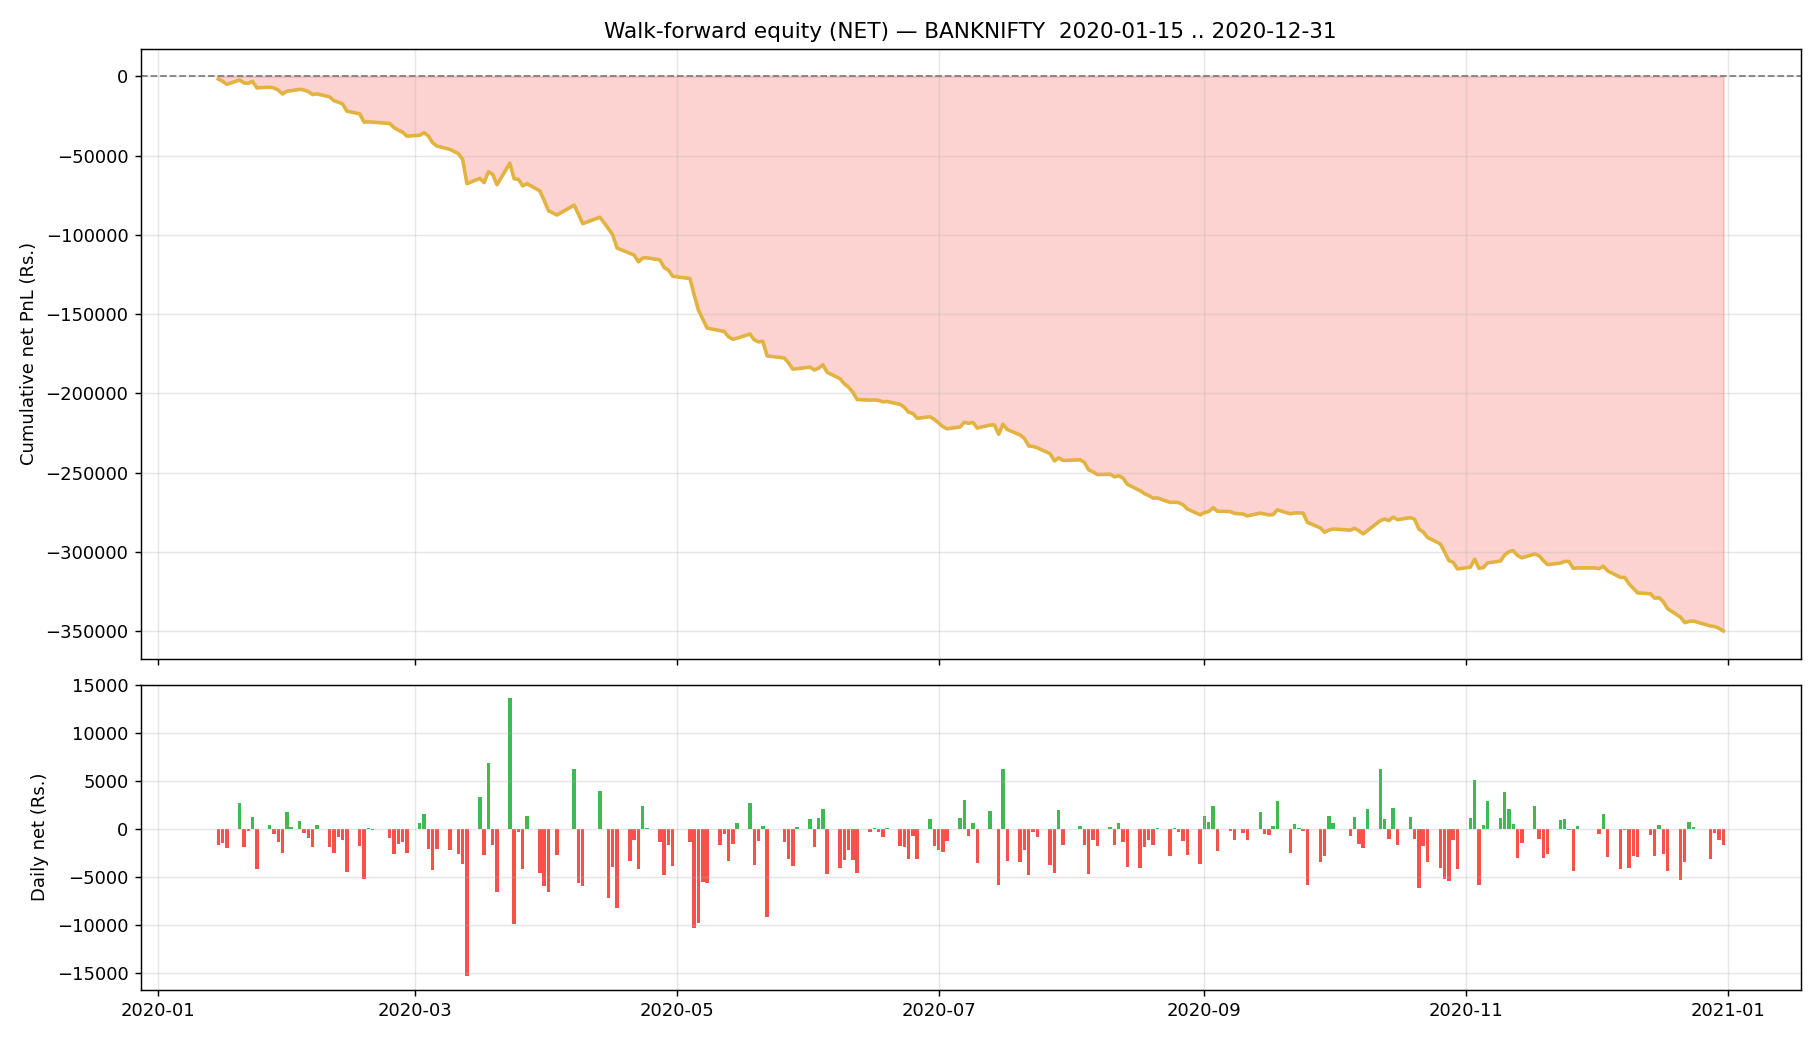
\includegraphics[width=0.92\textwidth]{fig01_baseline_equity.png}
\caption{Phase 2 baseline, full-year 2020: cumulative net equity (top) and daily net
P\&L (bottom). The monotone decline is the signature of a cost-dominated strategy ---
losses accrue smoothly with trade count rather than in event-driven clusters.
Source: \code{reports/walkforward\_banknifty\_20260706\_154902/equity.png}.}
\label{fig:baseline}
\end{figure}

\subsection{Calibration, automatic thresholds and abstention}

Adding the three decision-layer components of Section~\ref{sec:decision} --- isotonic
calibration, threshold selection by simulated net profit, and the no-edge abstention
rule --- changes the result by an order of magnitude at the 5-minute horizon: net P\&L
improves from \rs$-349{,}791$ to \rs$-22{,}250$, trade count falls from 4{,}706 to 470,
and 113 of 242 days are skipped. Critically, \emph{gross} P\&L turns positive
(\rs$+5{,}225$): once the system stops trading indiscriminately, the remaining trades
do have a small directional edge.

\subsection{Horizon experiments}\label{sec:horizon}

The cost hurdle is independent of the horizon while the expected absolute move grows with
it, so a longer horizon should improve the ratio of edge to cost --- up to the point
where an unmanaged long position starts to bleed theta and give back gains.
Table~\ref{tab:horizon} tests $h \in \{5,15,30\}$ on the full year 2020.

\begin{table}[H]
\centering\small
\begin{tabular}{@{}lrrrrrrr@{}}
\toprule
\textbf{Configuration} & \textbf{Trades} & \textbf{Gross} & \textbf{Charges} &
\textbf{Net} & \textbf{PF} & \textbf{Sharpe} & \textbf{Skipped}\\
\midrule
Phase 2 baseline ($h=5$, fixed $0.70$) & 4{,}706 & $-72{,}379$ & $277{,}412$
  & $-349{,}791$ & $0.70$ & $-7.58$ & --\\
Phase 3, $h=5$m   & 470 & $+5{,}225$ & $27{,}474$ & $-22{,}250$ & $0.79$ & $-2.60$ & 113\\
\textbf{Phase 3, $h=15$m} & \textbf{276} & $\mathbf{+5{,}710}$ & $\mathbf{15{,}693}$
  & $\mathbf{-9{,}983}$ & $\mathbf{0.85}$ & $\mathbf{-1.82}$ & 150\\
Phase 3, $h=30$m  & 236 & $-18{,}335$ & $13{,}936$ & $-32{,}271$ & $0.66$ & $-4.08$ & 153\\
\bottomrule
\end{tabular}
\caption{Horizon sweep, full-year 2020 (rupees). The 15-minute horizon is the optimum:
long enough to clear the cost hurdle, short enough that the position is not held into
decay. At $h=30$ the average loss grows to \rs$805$ against an average win of \rs$532$,
which is the signature of unmanaged long holds.}
\label{tab:horizon}
\end{table}

\begin{figure}[H]
\centering
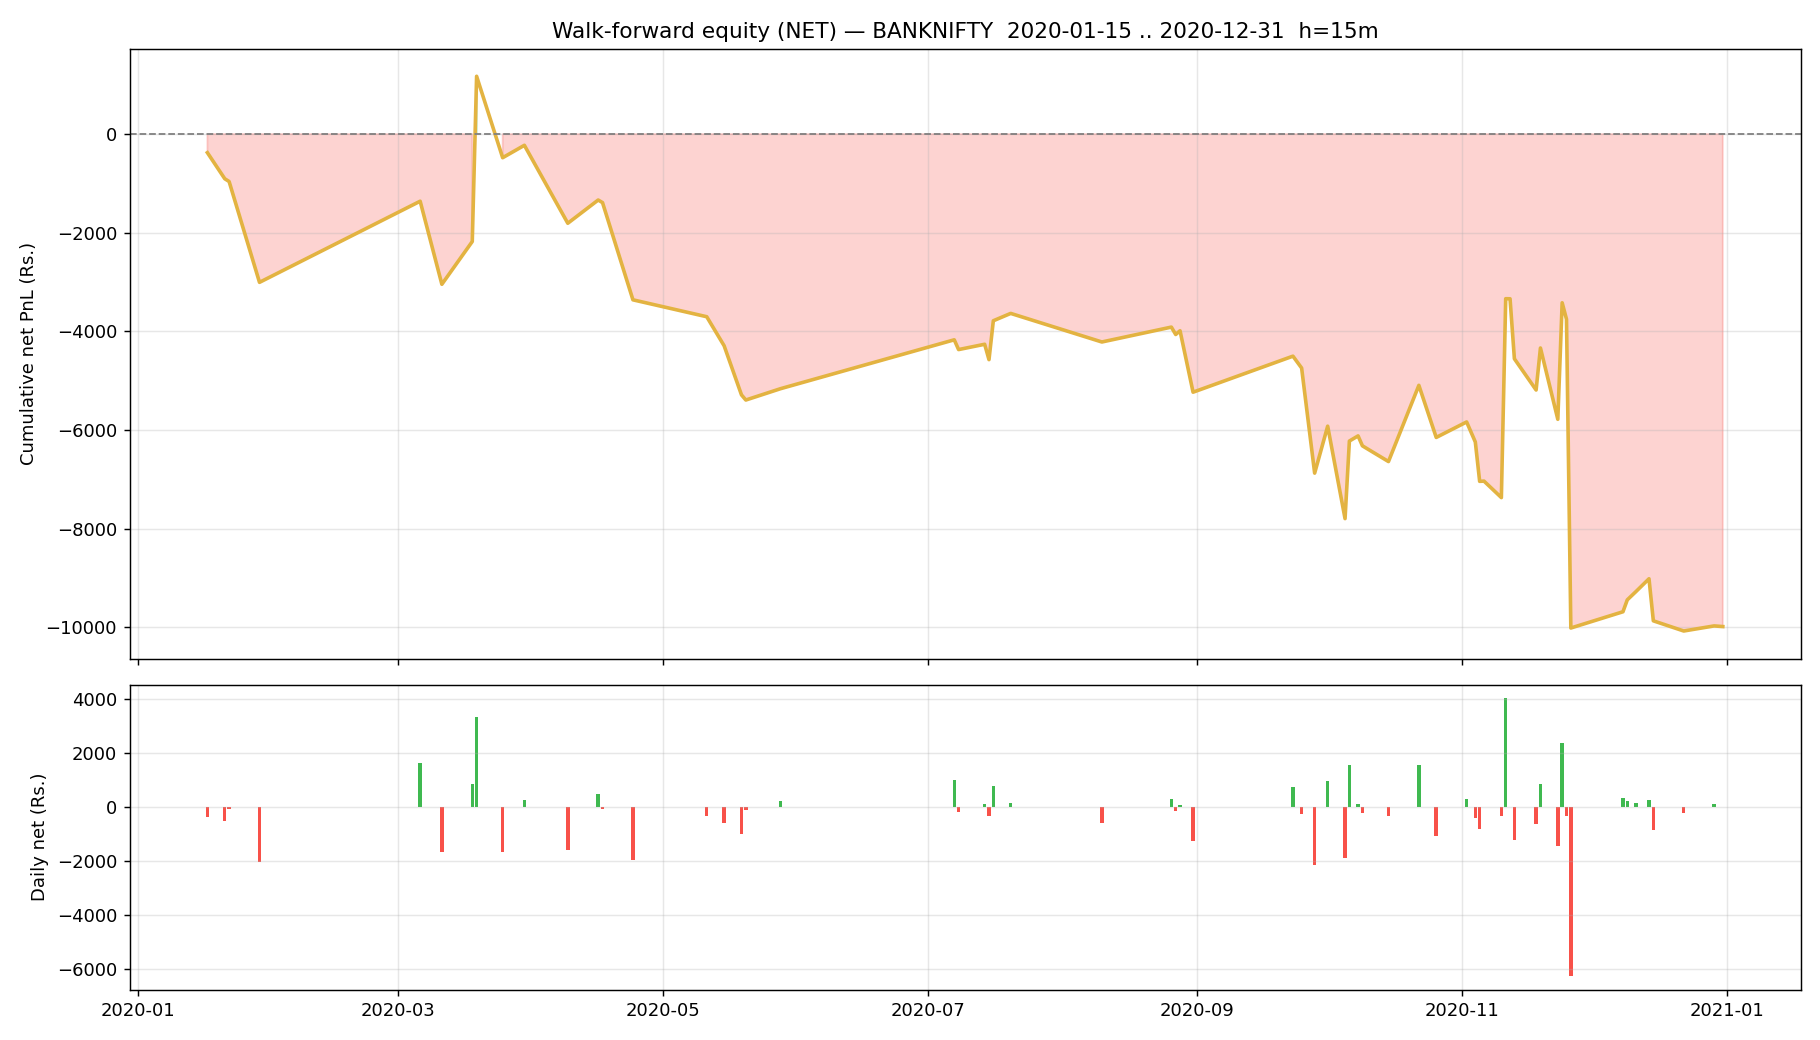
\includegraphics[width=0.92\textwidth]{fig02_h15_equity.png}
\caption{Best pre-risk-layer configuration ($h=15$m, calibrated, automatic threshold,
abstention), full-year 2020: 276 trades on 63 traded days, net \rs$-9{,}983$ with
\emph{positive} gross P\&L. Flat segments are skipped days.
Source: \code{reports/walkforward\_banknifty\_20260706\_162404/equity.png}.}
\label{fig:h15}
\end{figure}

\subsection{Risk-layer ablation}

We then added the risk layer and ablated its two contentious components --- stop width
and maximum position size --- on two independent years. Results are in
Table~\ref{tab:ablation}.

\begin{table}[H]
\centering\small
\begin{tabular}{@{}lrrrr@{}}
\toprule
\textbf{Configuration ($h=15$m)} & \textbf{2020 net} & \textbf{2021 net}
& \textbf{2020 trades} & \textbf{2021 trades}\\
\midrule
No risk layer (reference)                    & $-9{,}983$  & --          & 276 & --\\
$12\%$ stop, $\le 3$ lots, grid from $0.60$  & $-39{,}734$ & $-16{,}863$ & 144 & 167\\
$30\%$ stop, $\le 3$ lots, grid from $0.65$  & $-18{,}728$ & $-11{,}405$ & 91  & 99\\
$30\%$ stop, $1$ lot (final)                 & $-12{,}311$ & $-16{,}456$ & 97  & 103\\
\bottomrule
\end{tabular}
\caption{Risk-layer ablation on two independent years (rupees, net of all costs). The
tight stop is unambiguously harmful in both years; the remaining variants differ by less
than the year-to-year variation, and the sign of the difference flips between years.}
\label{tab:ablation}
\end{table}

\subsection{Where the money is made and lost: exit-reason decomposition}\label{sec:stops}

Table~\ref{tab:exits} is the single most informative table in this paper. It decomposes
net profit by the reason the position was closed.

\begin{table}[H]
\centering\small
\begin{tabular}{@{}llrrr@{}}
\toprule
\textbf{Run} & \textbf{Exit reason} & \textbf{Count} & \textbf{Mean (\rs)} & \textbf{Sum (\rs)}\\
\midrule
2020, $12\%$ stop & signal & 55 & $+147.0$ & $+8{,}083$\\
                  & target & 10 & $+1{,}586.3$ & $+15{,}863$\\
                  & time   & 12 & $+115.8$ & $+1{,}389$\\
                  & \textbf{stop} & \textbf{65} & $\mathbf{-996.0}$ & $\mathbf{-64{,}738}$\\
\midrule
2021, $12\%$ stop & signal & 90 & $+256.3$ & $+23{,}067$\\
                  & target &  8 & $+1{,}414.9$ & $+11{,}319$\\
                  & time   & 19 & $-4.4$ & $-85$\\
                  & \textbf{stop} & \textbf{50} & $\mathbf{-1{,}023.3}$ & $\mathbf{-51{,}164}$\\
\midrule
2020, $30\%$ stop, 1 lot & signal & 47 & $+46.4$ & $+2{,}183$\\
                  & target & 11 & $+585.4$ & $+6{,}439$\\
                  & time   & 28 & $-353.2$ & $-9{,}891$\\
                  & stop   & 10 & $-1{,}076.6$ & $-10{,}766$\\
\midrule
2021, $30\%$ stop, 1 lot & signal & 71 & $-9.7$ & $-687$\\
                  & target &  5 & $+1{,}179.9$ & $+5{,}900$\\
                  & time   & 21 & $-532.1$ & $-11{,}175$\\
                  & stop   &  6 & $-1{,}749.0$ & $-10{,}494$\\
\bottomrule
\end{tabular}
\caption{Net profit by exit reason. With a $12\%$ stop, \emph{every other exit type is
net positive in both years} while stop-outs alone lose \rs$64{,}738$ (2020) and
\rs$51{,}164$ (2021) --- a combined \rs$115{,}902$ of self-inflicted damage.}
\label{tab:exits}
\end{table}

This is the empirical confirmation of the microstructure argument of
Section~\ref{sec:risk}: the stop was not protecting the strategy from losing trades, it
was converting ordinary intrabar noise into realised losses at approximately \rs$1{,}000$
per occurrence. Widening the stop to $30\%$ reduces stop-outs from 65 to 10 in 2020 and
moves the damage into the (much cheaper) time-exit bucket.

\begin{figure}[H]
\centering
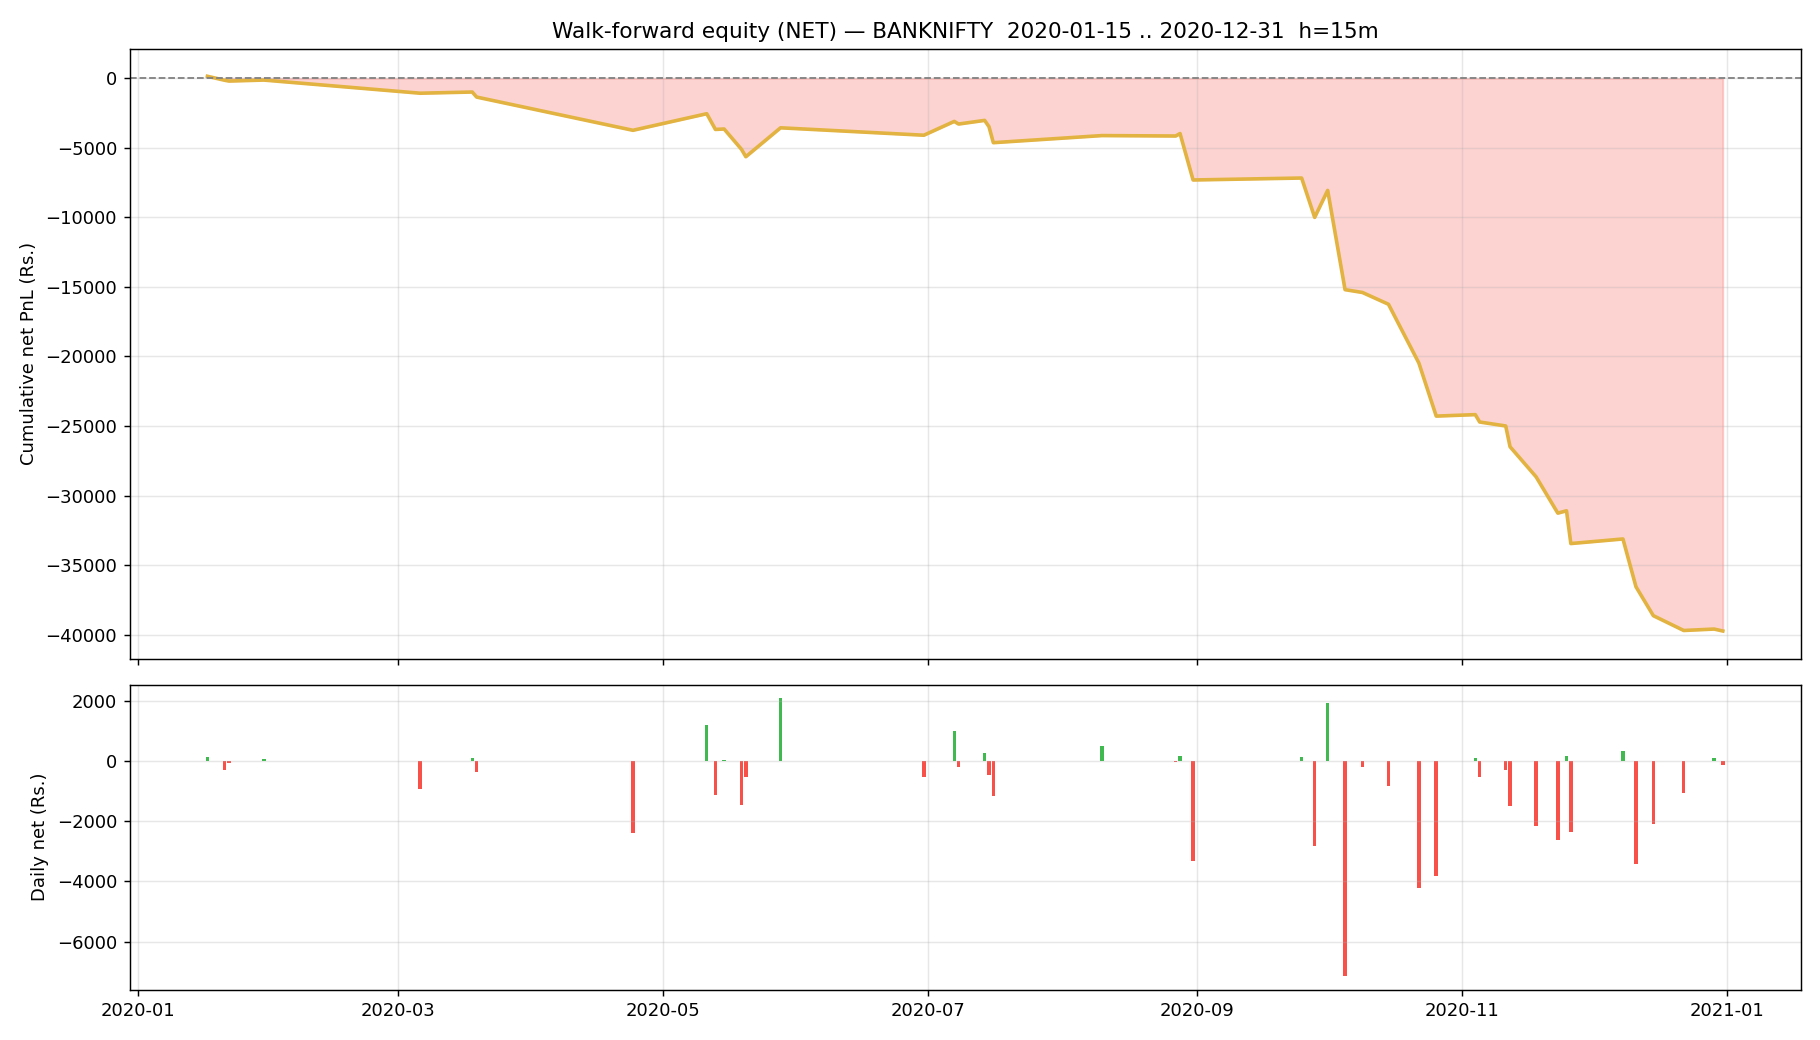
\includegraphics[width=0.92\textwidth]{fig03_stop12_equity.png}
\caption{The $12\%$-stop configuration, full-year 2020 (net \rs$-39{,}734$, profit
factor $0.44$). The steep drops are clusters of stop-outs; compare with
Figure~\ref{fig:h15}, the same signal without a tight stop.
Source: \code{reports/walkforward\_banknifty\_20260706\_165719/equity.png}.}
\label{fig:stop12}
\end{figure}

\subsection{Position size decomposition}\label{sec:sizing}

Table~\ref{tab:lots} decomposes the same runs by the number of lots the conviction ladder
selected.

\begin{table}[H]
\centering\small
\begin{tabular}{@{}lrrrrrr@{}}
\toprule
& \multicolumn{2}{c}{\textbf{1 lot}} & \multicolumn{2}{c}{\textbf{2 lots}}
& \multicolumn{2}{c}{\textbf{3 lots}}\\
\cmidrule(lr){2-3}\cmidrule(lr){4-5}\cmidrule(lr){6-7}
\textbf{Run} & Count & Net (\rs) & Count & Net (\rs) & Count & Net (\rs)\\
\midrule
2020, $12\%$ stop, $\le3$ lots & 86 & $-14{,}597$ & 40 & $-15{,}609$ & 18 & $-9{,}528$\\
2021, $12\%$ stop, $\le3$ lots & 103 & $-2{,}595$ & 45 & $-20{,}789$ & 19 & $+6{,}521$\\
2020, $30\%$ stop, $\le3$ lots & 49 & $-2{,}255$ & 30 & $-17{,}537$ & 12 & $+1{,}065$\\
2021, $30\%$ stop, $\le3$ lots & 63 & $-9{,}200$ & 26 & $-4{,}484$ & 10 & $+2{,}279$\\
\bottomrule
\end{tabular}
\caption{Net profit by position size. The multi-lot buckets carry a disproportionate
share of the loss, and the sign of the 3-lot bucket is inconsistent across years, which
is what a zero-edge signal looks like when amplified.}
\label{tab:lots}
\end{table}

The 2-lot bucket is the worst in three of four runs. This is Equation~\eqref{eq:sizing}
applied to a signal whose $\mu$ is not reliably positive: scaling multiplies a negative
expectancy and widens the outcome distribution. We therefore set $n_{\max}=1$ in the
final configuration.

\subsection{Final configuration}

The configuration carried forward is: $h = 15$ minutes, maximum hold 30 bars, isotonic
calibration, automatic threshold over $\{0.65,0.70,0.75,0.80\}$, abstention on days with
no measured edge, $30\%$ disaster stop, $24\%$ target, one lot, four trades per contract
per day, \rs$3{,}000$ daily loss limit, and the volatility band
$\text{rv}_{15} \in [0.02, 0.30]$.

\begin{table}[H]
\centering\small
\begin{tabular}{@{}lrr@{}}
\toprule
& \textbf{2020} & \textbf{2021}\\
\midrule
Test days (candidate)      & 242 & 238\\
Days skipped by abstention & 173 & 171\\
Days actually traded       & 38 & 30\\
Trades                     & 97 & 103\\
Win rate                   & $45.4\%$ & $43.7\%$\\
Gross P\&L (\rs)           & $-6{,}760$ & $-10{,}503$\\
Charges (\rs)              & $5{,}551$ & $5{,}954$\\
\textbf{Net P\&L (\rs)}    & $\mathbf{-12{,}311}$ & $\mathbf{-16{,}456}$\\
Expectancy per trade (\rs) & $-126.9$ & $-159.8$\\
Profit factor              & $0.61$ & $0.50$\\
Max drawdown (\rs)         & $13{,}912$ & $17{,}755$\\
Sharpe (annualised)        & $-4.63$ & $-6.64$\\
\bottomrule
\end{tabular}
\caption{Final Phase 2 configuration evaluated on two independent years.}
\label{tab:final}
\end{table}

\begin{figure}[H]
\centering
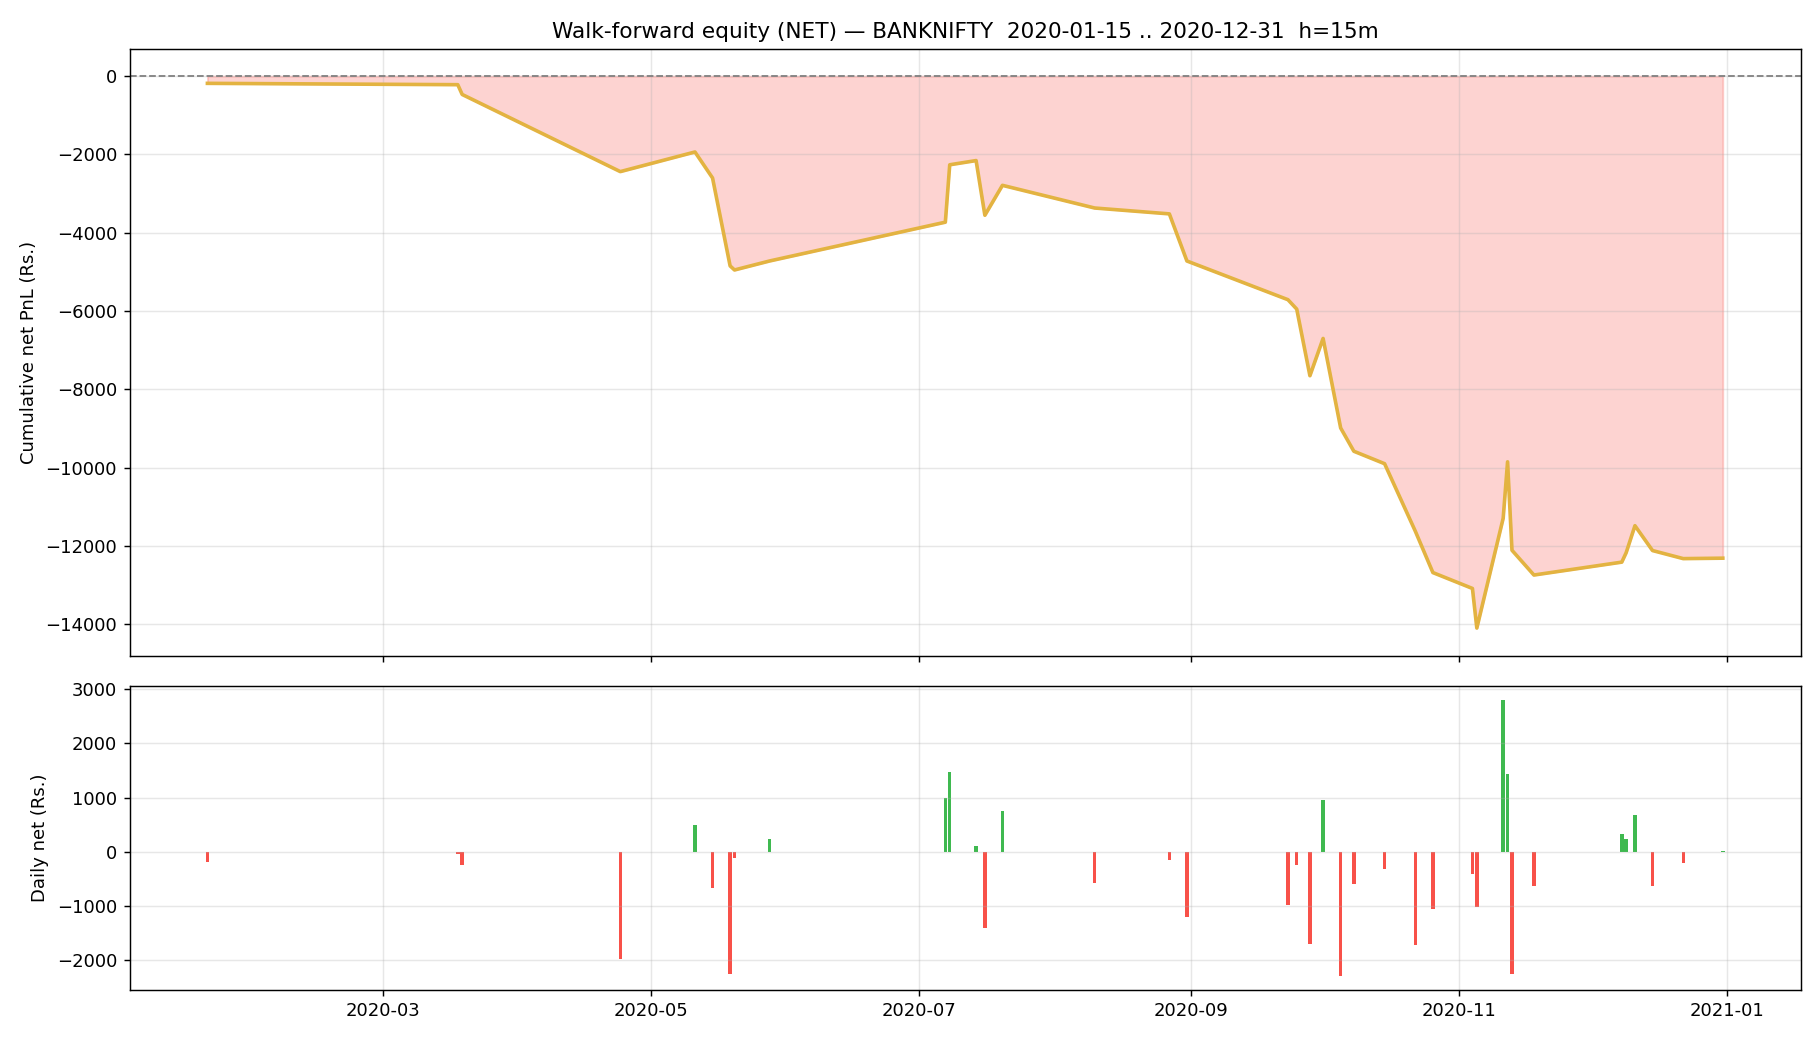
\includegraphics[width=0.92\textwidth]{fig04_final2020_equity.png}
\caption{Final configuration, 2020. Net \rs$-12{,}311$ over 97 trades on 38 traded days.
Source: \code{reports/walkforward\_banknifty\_20260706\_174950/equity.png}.}
\label{fig:final2020}
\end{figure}

\begin{figure}[H]
\centering
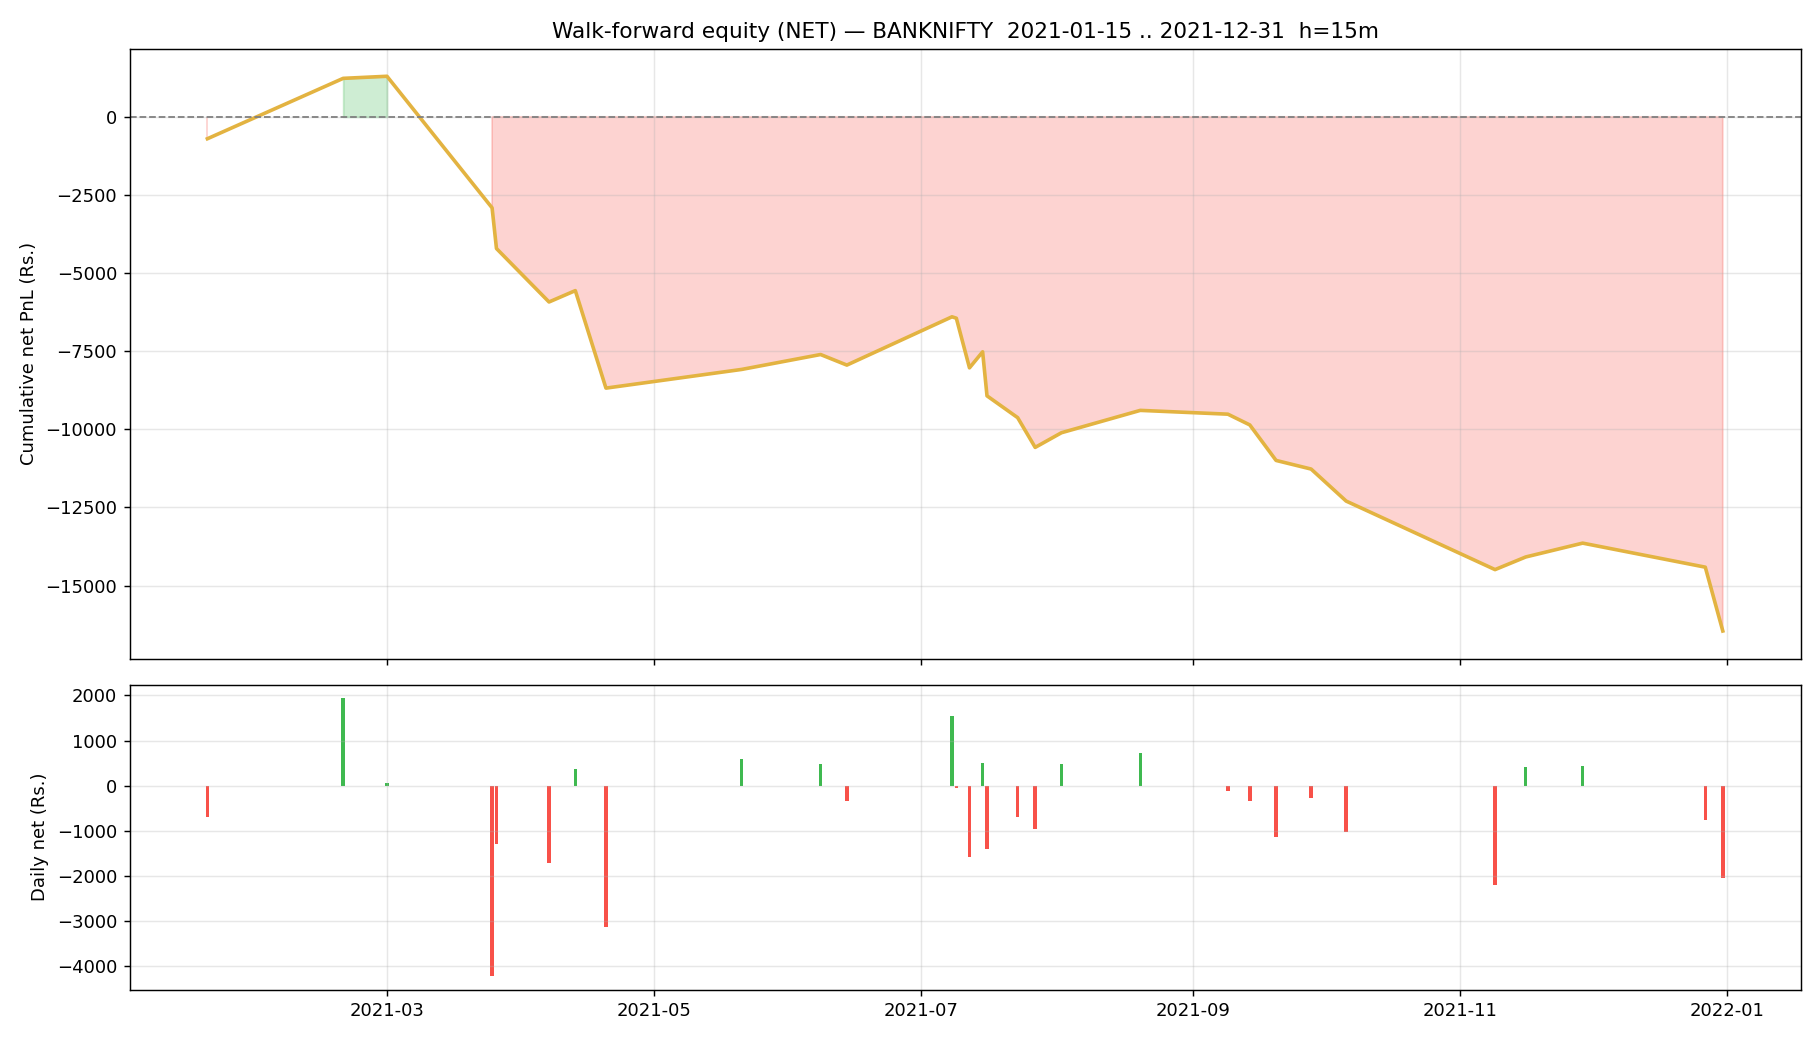
\includegraphics[width=0.92\textwidth]{fig05_final2021_equity.png}
\caption{Final configuration, 2021 --- an independent year with a different volatility
regime. Net \rs$-16{,}456$ over 103 trades. The similarity of the two years' magnitudes,
despite very different market conditions, is the basis of the noise-floor claim of
Section~\ref{sec:floor}.
Source: \code{reports/walkforward\_banknifty\_20260706\_180124/equity.png}.}
\label{fig:final2021}
\end{figure}

\subsection{Overall progression}

\begin{table}[H]
\centering\small
\begin{tabular}{@{}llrrr@{}}
\toprule
\textbf{Stage} & \textbf{What changed} & \textbf{Trades} & \textbf{Net 2020 (\rs)}
& \textbf{Improvement}\\
\midrule
Phase 1 (single day, no costs) & --- & 10 & not comparable & ---\\
Phase 2 baseline & costs, correct labels, full year & 4{,}706 & $-349{,}791$ & reference\\
+ calibration, auto threshold, abstention & $h=5$ & 470 & $-22{,}250$ & $15.7\times$\\
+ horizon 15m & $h=15$ & 276 & $-9{,}983$ & $35.0\times$\\
+ risk layer (final) & stops, caps, 1 lot & 97 & $-12{,}311$ & $28.4\times$\\
\bottomrule
\end{tabular}
\caption{Cumulative effect of the Phase 2 work on the same year of data. The strategy is
still not profitable; what improved by a factor of roughly 30 is the amount of money the
measurement apparatus was throwing away.}
\label{tab:progress}
\end{table}

%=======================================================================
\section{Discussion}\label{sec:discussion}
%=======================================================================

\subsection{Where the money goes}

At the best configuration ($h=15$, Table~\ref{tab:horizon}) charges were \rs$15{,}693$
over 276 trades, i.e.\ \rs$56.9$ per trade, of which \rs$40$ --- $70\%$ --- is flat
brokerage on two orders. The strategy's gross edge at that configuration was
\rs$+5{,}710$, or \rs$+20.7$ per trade. The arithmetic of the problem is therefore
stark and simple:
\begin{equation}
\underbrace{+20.7}_{\text{gross edge/trade}} \;-\;
\underbrace{40.0}_{\text{brokerage}} \;-\;
\underbrace{16.9}_{\text{statutory + slippage}} \;=\; -36.2\ \text{\rs/trade}.
\end{equation}
Two structural remedies follow, and neither is a machine-learning remedy: increase the
edge per trade (longer horizons, better signal, better entry timing), or increase the
position size over which the flat fee is amortised --- which, per Section~\ref{sec:sizing},
is only permissible once the edge is demonstrably positive.

\subsection{The noise floor}\label{sec:floor}

Across the post-ablation variants the results differ by roughly \rs$\pm 5{,}000$ per year
and the sign of the difference between configurations flips between 2020 and 2021
(Table~\ref{tab:ablation}). In other words, the remaining differences between execution
variants are not statistically distinguishable from year-to-year variation. We therefore
characterise the current state as a \emph{trade-management noise floor} of roughly
\rs$-10{,}000$ to \rs$-16{,}000$ per year: at this point additional tuning of stops,
targets, thresholds or session windows produces changes that are indistinguishable from
noise, and continuing to tune them would be fitting the configuration to two specific
years. The honest conclusion is that further gains must come from signal quality.

\subsection{The deadband--hurdle mismatch}\label{sec:hurdle-mismatch}

The most actionable finding of this paper emerged from writing it rather than from
running it. The model is trained to answer:
\[
\text{``Will the premium be more than } 0.1\% \text{ higher in 15 minutes?''}
\]
while the trading system needs an answer to:
\[
\text{``Will the premium be more than } \approx\!1.5\% \text{ higher before my stop or my
time limit?''}
\]
These are different questions, and the first is much easier than the second. A model that
answers the first with high skill can still lose money, because a $0.1\%$ move is
$15\times$ too small to pay for itself (Table~\ref{tab:hurdle}). The remedy is to align
the label with the decision:

\begin{enumerate}
  \item set $\delta \approx H$, i.e.\ make the deadband the cost hurdle, so that the
        positive class means ``profitable after costs''; or, better,
  \item adopt triple-barrier labelling \cite{lopezdeprado,darufinance}: label a sample
        $+1$ if the premium touches $+H'$ before touching $-\theta_{\text{sl}}$ within
        $\tau_{\max}$ bars, $-1$ if the reverse, and $0$ if the time barrier is hit first.
        This makes the label \emph{identical} to the trade the system will actually place.
\end{enumerate}
We state this as a falsifiable prediction for the next phase: raising the deadband
towards the cost hurdle will reduce the positive-class frequency sharply and should
increase net expectancy per trade, even if headline accuracy falls. If it does not, our
account of why the strategy loses money is wrong and must be revised.

\subsection{Abstention as a first-class strategy component}

In the final configuration the system declines to trade on $71\%$ of candidate days
(173 of 242 in 2020). This is not a defect but a result: on the majority of days a
10-day-trained model shows no measurable post-cost edge on the most recent two days, and
trading them would cost money. Interpreting abstention as information rather than as
failure is, in our view, the most transferable lesson of Phase 2 --- and it suggests that
future work should model the \emph{tradeability} of a day directly (a meta-model over
regime features), which is the meta-labelling idea in \cite{lopezdeprado}.

\subsection{Threats to validity}\label{sec:threats}

We list the limitations we consider material, in descending order of concern.

\begin{enumerate}
  \item \textbf{Multiple testing.} Thirteen full experiments are recorded in
        \code{experiments.csv}, and parameters (threshold grid, stop level, horizon,
        maximum lots) were chosen after seeing results on 2020 and 2021. Under repeated
        trials the best observed configuration is an upwardly biased estimate of true
        performance; the deflated Sharpe ratio exists precisely to correct for this
        \cite{deflatedsharpe,bailey}. Our defence is procedural, not statistical: the
        2022--2024 holdout has never been touched, and the final configuration must be
        evaluated there exactly once.
  \item \textbf{Fills are modelled, not observed.} Our dataset contains OHLC bars, not
        quotes. Entries and exits are assumed to occur at the bar close (or at the stop
        or target price) adjusted by a fixed $0.25\%$ slippage. Real spreads on BankNifty
        options vary with moneyness, time of day and volatility; a spread-aware fill model
        would likely make results worse, not better.
  \item \textbf{Intrabar path is unknown.} When a bar's range spans both the stop and the
        target we assume the stop is hit first. This is conservative but arbitrary; a
        tick-level reconstruction would settle it.
  \item \textbf{Lot sizes are approximate.} The step function in
        Appendix~\ref{app:config} was assembled from secondary sources and must be
        verified circular by circular \cite{nsecircular} before any live use; profit
        scales linearly with it.
  \item \textbf{Purging and embargoing are not implemented.} As discussed in
        Section~\ref{sec:decision}, label horizons can overlap the fit/calibration
        boundary by up to $h$ minutes.
  \item \textbf{Single instrument, two years.} All results are BankNifty 2020--2021.
        NIFTY features have not yet been built, and 2020 in particular contains the
        COVID-19 crash, an extreme volatility regime.
  \item \textbf{The abstention rule uses a two-day sample.} Its estimator of ``edge''
        is extremely noisy; its large measured benefit may partly reflect a reduction in
        exposure rather than genuine selection skill. A direct test --- abstaining at
        random on the same fraction of days --- is a cheap and necessary control
        experiment that we have not yet run.
\end{enumerate}

%=======================================================================
\section{What Remains: The Phase 3 Programme}\label{sec:future}
%=======================================================================

\subsection{A controlled multi-algorithm benchmark}\label{sec:benchmark}

The most frequently proposed next step within our team is to train several algorithms of
the same family and compare them. We endorse this, but only under a protocol strict
enough that the comparison means something. The risk is obvious: running six models and
reporting the best is exactly the multiple-testing failure described in
Section~\ref{sec:threats}. The following protocol is designed to avoid it.

\paragraph{Candidates.} Chosen to span a spectrum of capacity, with the linear model as
the honesty check:
\begin{table}[H]
\centering\small
\begin{tabular}{@{}llp{6.6cm}@{}}
\toprule
\textbf{Model} & \textbf{Reference} & \textbf{Why it is in the comparison}\\
\midrule
Logistic regression & --- & Floor model. If boosting cannot beat a regularised linear
model on identical features, the non-linearity is not earning its keep.\\
Random forest & --- & Variance-reduction ensemble; a different inductive bias from
boosting (bagged deep trees vs.\ sequential shallow trees).\\
LightGBM (incumbent) & \cite{lightgbm} & Current baseline; leaf-wise growth, histogram
binning, native NaN handling.\\
XGBoost & \cite{xgboost} & Level-wise growth with explicit regularisation; the standard
against which boosting implementations are compared.\\
CatBoost & \cite{catboost} & Ordered boosting, designed to remove the target leakage that
affects conventional boosting on small, noisy datasets --- plausibly relevant at our
sample sizes.\\
LSTM / temporal model & --- & Consumes the bar \emph{sequence} rather than a
snapshot row; tests whether temporal structure beyond our engineered lags exists.\\
\bottomrule
\end{tabular}
\caption{Proposed candidate models for the Phase 3 benchmark.}
\label{tab:candidates}
\end{table}

\paragraph{Controls.} Identical features, identical labels, identical walk-forward
windows, identical calibration procedure, identical cost model, identical risk
configuration, identical random seeds. The \emph{only} thing that varies is the
estimator. Any hyperparameter search must occur strictly inside the training window of
each fold, never across folds.

\paragraph{Metrics, reported in two layers.} Statistical quality first: AUC (ranking),
log-loss and Brier score (probability quality), and calibration curves. Economic quality
second: net P\&L, expectancy per trade, profit factor, annualised Sharpe, maximum
drawdown and number of traded days. A model may win on AUC and lose on net P\&L; that
divergence is itself a finding, and Section~\ref{sec:hurdle-mismatch} predicts it will
occur if the label remains misaligned with the cost hurdle.

\paragraph{Selection discipline.} Select on 2020--2021 only. Then evaluate the single
selected model on 2022--2024 exactly once. Report the deflated Sharpe ratio
\cite{deflatedsharpe} alongside the raw Sharpe, using the number of configurations tried
as the trial count, so that the selection bias is quantified rather than hidden.

\paragraph{Beyond picking a winner.} Two extensions are cheap and often more informative
than the comparison itself: (i) an \emph{ensemble} that averages calibrated
probabilities across models, which usually improves calibration even when it does not
improve AUC; and (ii) a \emph{disagreement filter} that trades only when the models
agree, converting model variance into an abstention signal of the kind that already
works well for us.

\subsection{Label redesign}

Implement triple-barrier labelling with the upper barrier set at the measured cost hurdle
(Section~\ref{sec:hurdle-mismatch}), and re-run the entire pipeline unchanged. This is
the highest-expected-value experiment available to us, because it is the only one that
addresses the identified mismatch between what the model learns and what the system needs.

\subsection{Event and news risk (the ``war factor'')}

The system currently has no notion of why a day is dangerous. We will add a single
quantity $\text{event\_risk}\in[0,1]$ with a category (war/geopolitics, policy, election,
budget, crash), produced by two inputs: a manual operator dial in a hot-reloaded
configuration file, and an automatic news reader that polls RSS headlines, scores them
with a rule-based tier and an LLM-based tier, and aggregates them with exponential time
decay. It will be consumed both as a risk overlay (reduce size, raise the threshold, or
halt entries) and as a model feature, measured separately. The layer will be backtested
on labelled historical events (the COVID-19 crash of March 2020, the Russia--Ukraine
escalation of February 2022, the 2024 general election) with India VIX as a continuous
proxy, and judged on drawdown reduction rather than on profit.

\subsection{Simulated live execution}

A replay feed that streams a historical day bar by bar, a paper broker that fills orders
at the next bar with the Phase 2 cost model, an orchestrator that runs the identical loop
used in the backtest, and a dashboard showing price, probability, position, P\&L and the
event dial. The acceptance test is exact: replaying a day through the live loop must
reproduce the batch backtest for that day within slippage tolerance. Only then is the
distinction between ``backtest'' and ``system'' eliminated.

\subsection{Live market integration}

Fyers API v3 \cite{fyers,fyerswebsocket} provides OAuth authentication, a WebSocket feed
and order placement behind the same broker interface. The staged rollout is: live data
with paper broker for at least two weeks, then live trading at minimum size, then scaling
subject to demonstrated positive expectancy. Safety interlocks (market-hours check,
maximum order size, panic-flatten command, mandatory kill-switch test) precede the first
live order.

\subsection{Strategy-level alternatives}

If the long-options edge remains negative after the above, the same infrastructure
evaluates structurally different strategies without code changes: vertical spreads (which
cap both risk and cost per unit of exposure), shorter-dated expiry selection, and
NIFTY/BankNifty portfolio allocation. This is the argument for having built a framework
rather than a script: a negative result on one strategy costs a configuration change, not
a rewrite.

%=======================================================================
\section{Conclusion}
%=======================================================================

Phase 1 produced a model. Phase 2 produced a measurement instrument, and then used it to
measure the model honestly. The instrument found, in order: a labelling defect that had
been silently inflating accuracy; a cost structure that requires a $1$--$3\%$ move per
round trip and therefore invalidates high-frequency trading of cheap contracts; a raw
directional edge statistically indistinguishable from zero at a 5-minute horizon; a small
but positive gross edge at 15 minutes; a stop-loss rule that destroyed \rs$116{,}000$
across two years by harvesting microstructure noise; and a position-sizing rule that
amplified a negative expectancy. Removing these defects improved full-year 2020 net P\&L
from \rs$-349{,}791$ to \rs$-9{,}983$ --- a $35\times$ reduction --- while reducing
trade count from 4{,}706 to 276.

The strategy is not profitable. We consider the result nonetheless successful, for three
reasons. First, the improvement is attributable, component by component, to identified
defects rather than to parameter search. Second, the system now reports results that we
believe: every figure in this paper is net of statutory charges and modelled slippage,
computed on data the model had never seen at decision time. Third, the work produced a
specific, falsifiable hypothesis --- that the training label ($0.1\%$) is misaligned with
the economic hurdle ($\approx 1.5\%$) --- which is testable in a single experiment and
which, if confirmed, explains the residual gap.

The honest expectation stated at the start of Phase 2 stands: minute-level long-options
scalping is among the hardest edges in the market, because the trader pays theta, spread
and a flat fee on every attempt, and because $93\%$ of individual participants in this
segment lose money \cite{sebi}. What we can claim is that this project now measures that
difficulty correctly rather than hiding it, and that the same infrastructure will
evaluate the next hypothesis --- a realigned label, a different algorithm, an event-aware
risk overlay, or a spread strategy --- in hours rather than in weeks.

\appendix

%=======================================================================
\section{Configuration}\label{app:config}
%=======================================================================

\begin{lstlisting}[language=Python,caption={Excerpt of \code{config/settings.yaml} for the
final configuration.}]
instruments:
  banknifty:
    strike_step: 100
    lot_sizes:              # step function L(t); verify against NSE circulars
      2020-01-01: 20
      2021-07-30: 25
      2023-07-28: 15
      2024-11-20: 30

model:
  horizon_minutes: 15       # h
  moneyness_low: 0.85       # near-ATM band
  moneyness_high: 1.15
  min_premium: 5.0          # see Section 5.5: too permissive, raise in Phase 3
  label_deadband_pct: 0.10  # delta -- see the hurdle mismatch, Section 12.3
  n_estimators: 400
  learning_rate: 0.05

costs:
  brokerage_per_order: 20.0 # B, flat, per executed order
  stt_sell_pct: 0.0625      # sell-side premium turnover
  exchange_txn_pct: 0.05
  gst_pct: 18.0
  sebi_fee_pct: 0.0001
  stamp_duty_buy_pct: 0.003
  slippage_pct: 0.25        # per side, applied to the fill

strategy:
  exit_threshold: 0.45
  max_hold_bars: 30         # 2h
  trade_option_types: [CE, PE]
  threshold_grid: [0.65, 0.70, 0.75, 0.80]   # 0.60 removed: worst bucket both years

risk:
  stop_loss_pct: 30.0       # disaster stop only (12% harvested noise)
  take_profit_pct: 24.0
  base_lots: 1
  max_lots: 1               # earn the right to size up
  conviction_step: 0.06
  max_position_premium: 20000
  max_trades_per_day: 4
  daily_loss_limit: 3000
  no_entry_first_min: 5
  no_entry_after: "15:00"
  min_rv_15m: 0.02
  max_rv_15m: 0.30
\end{lstlisting}

%=======================================================================
\section{Reproduction}\label{app:repro}
%=======================================================================

\begin{lstlisting}[language=bash,caption={Commands that generated the reported runs.}]
# one-time: build the parquet feature store
python scripts/build_features.py --start 2020-01-01 --end 2024-12-31

# Phase 2 baseline (Table 5)
python scripts/run_walkforward.py --start 2020-01-01 --end 2020-12-31 \
       --entry 0.70 --exit 0.35 --no-calibrate --no-risk

# horizon sweep (Table 6)
python scripts/run_walkforward.py --start 2020-01-01 --end 2020-12-31 --horizon 5
python scripts/run_walkforward.py --start 2020-01-01 --end 2020-12-31 --horizon 15
python scripts/run_walkforward.py --start 2020-01-01 --end 2020-12-31 --horizon 30

# final configuration, two years (Table 10)
python scripts/run_walkforward.py --start 2020-01-01 --end 2020-12-31 --horizon 15
python scripts/run_walkforward.py --start 2021-01-01 --end 2021-12-31 --horizon 15

# test suite
pytest -q
\end{lstlisting}

%=======================================================================
\section{Test Suite}\label{app:tests}
%=======================================================================

\begin{table}[H]
\centering\small
\begin{tabular}{@{}lp{9.2cm}@{}}
\toprule
\textbf{File} & \textbf{What it proves}\\
\midrule
\code{test\_symbol\_parsing.py} & The regular expression decomposes
\code{BANKNIFTY16JAN2032200CE} into underlying, expiry, strike and option type.\\
\code{test\_targets.py} & Labels for contract $X$ never use prices of contract $Y$; the
gap guard invalidates labels across quote gaps; the deadband behaves as specified.\\
\code{test\_costs.py} & Round-trip charges match a hand-computed example; slippage moves
the fill against the trader on both sides.\\
\code{test\_config\_and\_loader.py} & \code{lot\_size\_for} returns the value in force on
a given date, including at boundaries.\\
\code{test\_calibration.py} & The isotonic map is monotone, preserves ranking (hence
AUC), and is skipped when the calibration fold is too small or single-class.\\
\code{test\_risk.py} & Each entry gate vetoes for the stated reason; the conviction
ladder respects both \code{max\_lots} and the premium cap; the daily kill-switch
triggers.\\
\bottomrule
\end{tabular}
\caption{The pytest suite (8 risk tests among 30 total assertions of behaviour).}
\end{table}

%=======================================================================
\begin{thebibliography}{99}
%=======================================================================

\bibitem{phase1} A.~Raj, S.~Singh, H.~R.~Sharma and N.~Das,
\emph{Phase 1 Comprehensive Theory Paper: Architecture, Methodology, and Iterative
Evolution of an AI-Driven NSE BankNifty Options Trading System}, May 2026.
(Submitted; attached as the companion document to this report.)

\bibitem{blackscholes} F.~Black and M.~Scholes,
``The Pricing of Options and Corporate Liabilities,''
\emph{Journal of Political Economy}, vol.~81, no.~3, pp.~637--654, 1973.
\href{https://doi.org/10.1086/260062}{Link: Journal of Political Economy (DOI)}

\bibitem{merton} R.~C.~Merton,
``Theory of Rational Option Pricing,''
\emph{Bell Journal of Economics and Management Science}, vol.~4, no.~1, pp.~141--183, 1973.
\href{https://doi.org/10.2307/3003143}{Link: Bell Journal of Economics (DOI)}

\bibitem{letsberational} P.~J\"ackel, ``Let's Be Rational,'' 2015.
Source code and paper: \href{http://www.jaeckel.org/}{Link: jaeckel.org -- Let's Be Rational}
(implementation used via \code{py\_lets\_be\_rational}).

\bibitem{pyvollib} Vollib project, \emph{py\_vollib / py\_lets\_be\_rational}.
\href{https://github.com/vollib/py_lets_be_rational}{Link: GitHub -- vollib source} and
\href{https://vollib.org/documentation/python/0.1.5/}{Link: vollib documentation}

\bibitem{lightgbm} G.~Ke, Q.~Meng, T.~Finley, T.~Wang, W.~Chen, W.~Ma, Q.~Ye and
T.-Y.~Liu, ``LightGBM: A Highly Efficient Gradient Boosting Decision Tree,''
\emph{Advances in Neural Information Processing Systems (NeurIPS)}, pp.~3146--3154, 2017.
\href{https://proceedings.neurips.cc/paper/2017/file/6449f44a102fde848669bdd9eb6b76fa-Paper.pdf}{Link: NeurIPS proceedings (PDF)}

\bibitem{xgboost} T.~Chen and C.~Guestrin, ``XGBoost: A Scalable Tree Boosting System,''
\emph{Proc. 22nd ACM SIGKDD}, 2016. \href{https://arxiv.org/abs/1603.02754}{Link: arXiv:1603.02754}

\bibitem{catboost} L.~Prokhorenkova, G.~Gusev, A.~Vorobev, A.~V.~Dorogush and A.~Gulin,
``CatBoost: Unbiased Boosting with Categorical Features,''
\emph{NeurIPS}, 2018. \href{https://arxiv.org/pdf/1706.09516}{Link: arXiv:1706.09516 (PDF)}

\bibitem{zadrozny} B.~Zadrozny and C.~Elkan,
``Transforming Classifier Scores into Accurate Multiclass Probability Estimates,''
\emph{Proc. 8th ACM SIGKDD}, pp.~694--699, 2002.
\href{https://dl.acm.org/doi/10.1145/775047.775151}{Link: ACM Digital Library}

\bibitem{sklearncalib} scikit-learn developers,
``1.16. Probability Calibration,'' \emph{scikit-learn User Guide}.
\href{https://scikit-learn.org/stable/modules/calibration.html}{Link: scikit-learn User Guide}

\bibitem{brier} scikit-learn developers, ``\code{brier\_score\_loss},''
\emph{scikit-learn API Reference}.
\href{https://scikit-learn.org/stable/modules/generated/sklearn.metrics.brier_score_loss.html}{Link: scikit-learn API reference}

\bibitem{lopezdeprado} M.~L\'opez de Prado,
\emph{Advances in Financial Machine Learning}. Wiley, 2018.
(Triple-barrier labelling, meta-labelling, purged cross-validation.)

\bibitem{purgedcv} ``Purged cross-validation,'' \emph{Wikipedia}.
\href{https://en.wikipedia.org/wiki/Purged_cross-validation}{Link: Wikipedia -- Purged cross-validation}

\bibitem{darufinance} Daru Finance, ``Labeling \& Cross-Validation, Purged CV,
Meta-Labeling \& Trend-Scanning.''
\href{https://daru.finance/research-review/lopez-de-prado/labeling-and-cross-validation}{Link: Daru Finance research review}

\bibitem{pardo} R.~E.~Pardo, ``Walk-Forward Analysis,'' in
\emph{The Evaluation and Optimization of Trading Strategies}, 2nd ed. Wiley, 2008.
\href{https://onlinelibrary.wiley.com/doi/abs/10.1002/9781119196969.ch11}{Link: Wiley Online Library}

\bibitem{wfowiki} ``Walk forward optimization,'' \emph{Wikipedia}.
\href{https://en.wikipedia.org/wiki/Walk_forward_optimization}{Link: Wikipedia -- Walk forward optimization}

\bibitem{deflatedsharpe} D.~H.~Bailey and M.~L\'opez de Prado,
``The Deflated Sharpe Ratio: Correcting for Selection Bias, Backtest Overfitting and
Non-Normality,'' \emph{Journal of Portfolio Management}, 2014.
\href{https://papers.ssrn.com/sol3/papers.cfm?abstract_id=2460551}{Link: SSRN abstract 2460551}

\bibitem{bailey} D.~H.~Bailey, J.~M.~Borwein, M.~L\'opez de Prado and Q.~J.~Zhu,
``Statistical Overfitting and Backtest Performance.''
\href{https://www.davidhbailey.com/dhbpapers/deflated-sharpe.pdf}{Link: davidhbailey.com (PDF)}

\bibitem{roll} R.~Roll,
``A Simple Implicit Measure of the Effective Bid--Ask Spread in an Efficient Market,''
\emph{The Journal of Finance}, vol.~39, no.~4, pp.~1127--1139, 1984.
\href{https://www.bauer.uh.edu/rsusmel/phd/roll1984.pdf}{Link: University of Houston (PDF)}

\bibitem{andersen} T.~G.~Andersen and T.~Bollerslev,
``Answering the Skeptics: Yes, Standard Volatility Models Do Provide Accurate Forecasts,''
\emph{International Economic Review}, vol.~39, no.~4, pp.~885--905, 1998.
\href{https://www.semanticscholar.org/paper/93ffc319bf39882dd471e1594ce242aee101ef38}{Link: Semantic Scholar}

\bibitem{sebi} Securities and Exchange Board of India,
``Updated SEBI Study Reveals 93\% of Individual Traders Incurred Losses in Equity F\&O
between FY22 and FY24,'' Press Release 22/2024, September 2024.
\href{https://www.sebi.gov.in/media-and-notifications/press-releases/sep-2024/updated-sebi-study-reveals-93-of-individual-traders-incurred-losses-in-equity-fando-between-fy22-and-fy24-aggregate-losses-exceed-1-8-lakh-crores-over-three-years_86906.html}{Link: SEBI media and notifications}

\bibitem{zerodhacharges} Zerodha, ``Brokerage charges, fees and taxes on trading and
investing.'' \href{https://zerodha.com/charges/}{Link: Zerodha charges}

\bibitem{zerodhastt} Zerodha Support,
``Securities Transaction Tax (STT): Rates and how to calculate it.''
\href{https://support.zerodha.com/category/account-opening/charges-at-zerodha/statutory-and-exchange/articles/how-is-the-securities-transaction-tax-stt-calculated}{Link: Zerodha support article}

\bibitem{nsecircular} National Stock Exchange of India,
``Revision in market lot of derivative contracts on indices,''
Circular NSE/FAOP/56233, 31 March 2023.
\href{https://archives.nseindia.com/content/circulars/FAOP56233.pdf}{Link: NSE circular FAOP56233 (PDF)}

\bibitem{iifl} IIFL Capital, ``Put Call Ratio: Nifty / Bank Nifty PCR.''
\href{https://www.indiainfoline.com/markets/derivatives/put-call-ratio}{Link: IIFL Capital}

\bibitem{groww} Groww, ``Advanced Option Chain Analysis: Strategies, Indicators \&
Insights.'' \href{https://groww.in/blog/advanced-option-chain}{Link: Groww blog}

\bibitem{pcrskeptic} Harbourfront Quantitative Research,
``Is the Put-Call Ratio a Reliable Predictor?''
\href{https://harbourfrontquant.substack.com/p/is-the-put-call-ratio-a-reliable}{Link: Harbourfront Quantitative Research}

\bibitem{parquet} Apache Software Foundation, \emph{Apache Parquet}.
\href{https://parquet.apache.org/}{Link: Apache Parquet}

\bibitem{fyers} Fyers, \emph{fyers-apiv3} Python client.
\href{https://pypi.org/project/fyers-apiv3/}{Link: PyPI -- fyers-apiv3}

\bibitem{fyerswebsocket} Fyers Support,
``How can I use the data-websocket in API v3 to access real-time data?''
\href{https://support.fyers.in/portal/en/kb/articles/how-can-i-use-the-data-websocket-in-api-v3-to-access-real-time-data}{Link: Fyers support article}

\end{thebibliography}

\end{document}
